%% USPSC-modelo.tex
% ---------------------------------------------------------------
% USPSC: Modelo de Trabalho Academico (tese de doutorado, dissertacao de
% mestrado e trabalhos monograficos em geral) em conformidade com 
% ABNT NBR 14724:2011: Informacao e documentacao - Trabalhos academicos -
% Apresentacao
%----------------------------------------------------------------
%% Esta é uma customização do abntex2-modelo-trabalho-academico.tex de v-1.9.5 laurocesar 
%% para as Unidades do Campus USP de São Carlos:
%% EESC - Escola de Engenharia de São Carlos
%% IAU - Instituto de Arquitetura e Urbanismo
%% ICMC - Instituto de Ciências Matemáticas e de Computação
%% IFSC - Instituto de Física de São Carlos
%% IQSC - Instituto de Química de São Carlos
%%
%% Este trabalho utiliza a classe USPSC.cls que é mantida pela seguinte equipe:
%% 
%% Programação:
%%   - Marilza Aparecida Rodrigues Tognetti - marilza@sc.usp.br (PUSP-SC)
%%   - Ana Paula Aparecida Calabrez - aninha@sc.usp.br (PUSP-SC)
%% Normalização e Padronização:
%%   - Brianda de Oliveira Ordonho Sigolo - brianda@usp.br (IAU)
%%   - Elena Luzia Palloni Gonçalves - elena@sc.usp.br (EESC)
%%   - Eliana de Cássia Aquareli Cordeiro - eliana@iqsc.usp.br (IQSC)
%%   - Flávia Helena Cassin - cassinp@sc.usp.br (EESC)
%%   - Maria Cristina Cavarette Dziabas - mcdziaba@ifsc.usp.br (IFSC)
%%   - Regina Célia Vidal Medeiros - rcvmat@icmc.usp.br (ICMC)
%%
%% O USPSC-modelo.tex utiliza:	
%%  USPSC.cls e USPSC1.cls
%% 	USPSC-modelo-references.bib
%%	USPSC-modelo.tex
%%	USPSC-unidades.tex
%%	Um dos arquivos com dados pre-textuais abaixo, em conformidade com a Unidade de vínculo do autor:
%%				USPSC-pre-textual-EESC.tex
%%				USPSC-pre-textual-IAU.tex
%%				USPSC-pre-textual-ICMC.tex
%%				USPSC-pre-textual-IFSC.tex
%%				USPSC-pre-textual-IQSC.tex
%%				USPSC-pre-textual-OUTRO.tex
%%	USPSC-fichacatalografica.tex ou fichacatalografica.pdf
%%	folhadeaprovacao.pdf
%%	USPSC-Cap1-Introducao.tex
%%	USPSC-Cap2-Desenvolvimento.tex
%%	USPSC-Cap3-Citacoes.tex
%%	USPSC-Cap4-referencias.tex
%%	USPSC-Cap5-Conclusao.tex
%%	USPSC-Apendices.tex
%%	USPSC-Anexos.tex
%%	USPSC-AcentuacaoLaTeX.tex
%%	USPSC-LetrasGregas.tex
%%	USPSC-SimbolosUteis.tex

%----------------------------------------------------------------
%% Sobre a classe abntex2.cls:
%% abntex2.cls, v-1.9.5 laurocesar
%% Copyright 2012-2015 by abnTeX2 group at https://www.abntex.net.br/ 
%%
%----------------------------------------------------------------

\documentclass[
% -- opções da classe memoir --
12pt,		% tamanho da fonte
openright,	% capítulos começam em pág ímpar (insere página vazia caso preciso)
twoside,  % para impressão em anverso (frente) e verso. Oposto a oneside - Nota: utilizar \imprimirfolhaderosto*
%oneside, % para impressão em páginas separadas (somente anverso) -  Nota: utilizar \imprimirfolhaderosto
% inclua uma % antes do comando twoside e exclua a % antes do oneside 
a4paper,			% tamanho do papel. 
% -- opções da classe abntex2 --
chapter=TITLE,		% títulos de capítulos convertidos em letras maiúsculas
% -- opções do pacote babel --
brazil,				% idioma adicional para hifenização
french,				% idioma adicional para hifenização
spanish,			% idioma adicional para hifenização
english				% o último idioma é o principal do documento
% {USPSC} configura o cabeçalho contendo apenas o número da página
]{USPSC}
%]{USPSC1}
% Inclua % antes de ]{USPSC} e retire a % antes de %]{USPSC1}
% para utilizar o cabeçalho diferenciado para as páginas pares e ímpares como indicado abaixo:
%- páginas ímpares: cabeçalho com seções ou subseções e o número da página
%- páginas pares: cabeçalho com o número da página e o título do capítulo 
% ---

% ---
% Pacotes básicos - Fundamentais 
% ---
\usepackage[T1]{fontenc}		% Seleção de códigos de fonte.
\usepackage[utf8]{inputenc}		% Codificação do documento (conversão automática dos acentos)
\usepackage{lmodern}			% Usa a fonte Latin Modern
% Para utilizar a fonte Times New Roman, inclua uma % no início do comando acima  "\usepackage{lmodern}"
% Abaixo, tire a % antes do comando  \usepackage{times}
%\usepackage{times}		    	% Usa a fonte Times New Roman	
% Lembre-se de alterar a fonte no comando que imprime o preâmbulo no arquivo da Classe USPSC.cls				
\usepackage{lastpage}			% Usado pela Ficha catalográfica
\usepackage{indentfirst}		% Indenta o primeiro parágrafo de cada seção.
\usepackage{color}				% Controle das cores
\usepackage{graphicx}			% Inclusão de gráficos
\usepackage{float} 				% Fixa tabelas e figuras no local exato
\usepackage{chemfig,chemmacros}	% Para escrever reações químicas
\usepackage{microtype} 			% para melhorias de justificação
\usepackage{pdfpages}
\usepackage{makeidx}           % para gerar índice remissimo

\usepackage[super]{nth}			% escrever numeros ordinarios sobrescritos
\usepackage{listings}			% escrever algoritmos
\usepackage{subcaption}			% construir subfiguras

\usepackage{xr}					% referencia de equacoes de outros capitulos
\externaldocument{USPSC-Cap2-Desenvolvimento.tex}

\usepackage{color, colortbl}
\definecolor{LightCyan}{rgb}{0.88,1,1}
\definecolor{Purple}{rgb}{0.5,0.5,1}
\usepackage[first=0,last=9]{lcg}

\usepackage{multirow}
% ---

% ---
% Pacotes de citações
% Citações padrão ABNT
% ---
% Sistemas de chamada: autor-data ou numérico.
% Sistema autor-data
\usepackage[alf,abnt-emphasize=bf, abnt-thesis-year=both, abnt-repeated-author-omit=yes, abnt-last-names=abnt, abnt-etal-cite,abnt-etal-list=3, abnt-etal-text=default, abnt-and-type=e, abnt-doi=doi, abnt-url-package=none, abnt-verbatim-entry=no]{abntex2cite}

% Para o IQSC, que indica todos os autores nas referências, incluir % no início do comando acima e retirar a % do comando abaixo 

%\usepackage[alf,abnt-emphasize=bf, abnt-thesis-year=both, abnt-repeated-author-omit=yes, abnt-last-names=abnt, abnt-etal-cite,abnt-etal-list=0, abnt-etal-text=default, abnt-and-type=e]{abntex2cite}

% Sistema Numérico
% Para citações numéricas, sistema adotado pelo IFSC, incluir % no início do comando acima e retirar a % do comando abaixo 
%\usepackage[num,overcite,abnt-emphasize=bf, abnt-thesis-year=both, abnt-repeated-author-omit=yes, abnt-last-names=abnt, abnt-etal-cite,abnt-etal-list=0, abnt-etal-text=default, abnt-and-type=e]{abntex2cite}

% Complementarmente, verifique as instruções abaixo sobre os Pacotes de Nota de rodapé
% ---
% Pacotes de Nota de rodapé
% Configurações de nota de rodapé

% O presente modelo adota o formato numérico para as notas de rodapés quando utiliza o sistema de chamada autor-data para citações e referências. Para utilizar o sistema de chamada numérico para citações e referências, habilitar um dos comandos abaixo.
% Há diversa opções para nota de rodapé no Sistema Numérico.  Para o IFSC, habilitade o comando abaixo.

%\renewcommand{\thefootnote}{\fnsymbol{footnote}}  %Comando para inserção de símbolos em nota de rodapé

% Outras opções para nota de rodapé no Sistema Numérico:
%\renewcommand{\thefootnote}{\alph{footnote}}      %Comando para inserção de letras minúscula em nota de rodapé
%\renewcommand{\thefootnote}{\Alph{footnote}}      %Comando para inserção de letras maiúscula em nota de rodapé
%\renewcommand{\thefootnote}{\roman{footnote}}     %Comando para inserção de números romanos minúsculos  em nota de rodapé
%\renewcommand{\thefootnote}{\Roman{footnote}}     %Comando para inserção de números romanos minúsculos  em nota de rodapé

\renewcommand{\footnotesize}{\small} %Comando para diminuir a fonte das notas de rodapé

 % ---
 % Pacote para agrupar a citação numérica consecutiva
 % Quando for adotado o Sistema Numérico, a exemplo do IFSC, habilite 
 % o pacote cite abaixo retirando a porcentagem antes do comando abaixo
 %\usepackage[superscript]{cite}	

% ---
% Pacotes adicionais, usados apenas no âmbito do Modelo Canônico do abnteX2
% ---
\usepackage{lipsum}				% para geração de dummy text
% ---




% pacotes de tabelas
\usepackage{multicol}	% Suporte a mesclagens em colunas
\usepackage{multirow}	% Suporte a mesclagens em linhas
\usepackage{longtable}	% Tabelas com várias páginas
\usepackage{threeparttablex}    % notas no longtable
\usepackage{array}

%---
% Configurações para o pacote chemfig
%\chemsetup[chemformula]{format=\sffamily}
\renewcommand*\printatom[1]{\ensuremath{\mathsf{#1}}}
\setatomsep{2em}
\setdoublesep{.6ex}
\setbondstyle{semithick}
%---
% Configurando o ambiente para utilizar os recursos de frases pre-prontas do mhchem
\newenvironment{rslist}%
{%
	\begin{labeling}% environment from KOMA-script
		{\rsnumber{R39/23/24/25}}% R39/23/24/25 is longest label
	}{%
\end{labeling}%
}%
% Definição de comando para utilizar os recursos de frases pre-prontas do mhchem
\newcommand{\rs}[2][]{\item[{\rsnumber[#1]{#2}}] \rsphrase{bb}}
% ---

% ---
% DADOS INICIAIS - Define sigla com título, área de concentração e opção do Programa 
% Consulte a tabela referente aos Programas, áreas e opções de sua unidade contante do
% arquivo USPSC-Siglas estabelecidas para os Programas de Pós-Graduação por Unidade.xlsx 
% ou nos APÊNDICES A-E
\siglaunidade{EESC}
\programa{MEEE}
% Os demais dados deverão ser fornecidos no arquivo USPSC-pre-textual-UUUU, onde UUUU é a sigla da Unidade. 
% Exemplo:USPSC-pre-textual-IFSC.tex
% ---
% Configurações de aparência do PDF final
% alterando o aspecto da cor azul
\definecolor{blue}{RGB}{41,5,195}

% informações do PDF
\makeatletter
\hypersetup{
	%pagebackref=true,
	pdftitle={\@title}, 
	pdfauthor={\@author},
	pdfsubject={\imprimirpreambulo},
	pdfcreator={LaTeX with abnTeX2},
	pdfkeywords={abnt}{latex}{abntex}{USPSC}{trabalho acadêmico}, 
	colorlinks=true,       		% false: boxed links; true: colored links
	linkcolor=blue,          	% color of internal links
	citecolor=blue,        		% color of links to bibliography
	filecolor=magenta,      		% color of file links
	urlcolor=blue,
	bookmarksdepth=4
}
\makeatother
% --- 
% --- 
% Espaçamentos entre linhas e parágrafos 
% --- 

% O tamanho do parágrafo é dado por:
\setlength{\parindent}{1.3cm}

% Controle do espaçamento entre um parágrafo e outro:
\setlength{\parskip}{0.2cm}  % tente também \onelineskip

% ---
% compila o sumário e índice
\makeindex
% ---

% ----
% Início do documento
% ----
\begin{document}

% Seleciona o idioma do documento (conforme pacotes do babel)
%\selectlanguage{brazil}
% Se o idioma do texto for inglês, inclua uma % antes do 
%      comando \selectlanguage{brazil} e 
%      retire a % antes do comando abaixo
\selectlanguage{english}

% Retira espaço extra obsoleto entre as frases.
\frenchspacing 

% --- Formatação dos Títulos
\renewcommand{\ABNTEXchapterfontsize}{\fontsize{12}{12}\bfseries}
\renewcommand{\ABNTEXsectionfontsize}{\fontsize{12}{12}\bfseries}
\renewcommand{\ABNTEXsubsectionfontsize}{\fontsize{12}{12}\normalfont}
\renewcommand{\ABNTEXsubsubsectionfontsize}{\fontsize{12}{12}\normalfont}
\renewcommand{\ABNTEXsubsubsubsectionfontsize}{\fontsize{12}{12}\normalfont}


% ----------------------------------------------------------
% ELEMENTOS PRÉ-TEXTUAIS
% ----------------------------------------------------------
% ---
% Capa
% ---
\imprimircapa
% ---
% Folha de rosto
% (o * indica impressão em anverso (frente) e verso )
% ---
\imprimirfolhaderosto*
%\imprimirfolhaderosto
% ---

% ---
% Inserir a ficha catalográfica em pdf
% ---
% A biblioteca da sua Unidade lhe fornecerá um PDF com a ficha
% catalográfica definitiva. 
% Quando estiver com o documento, salve-o como PDF no diretório
% do seu projeto como fichacatalografica.pdf e iclua o arquivo
% utilizando o comando abaixo:

%\begin{fichacatalografica}
%   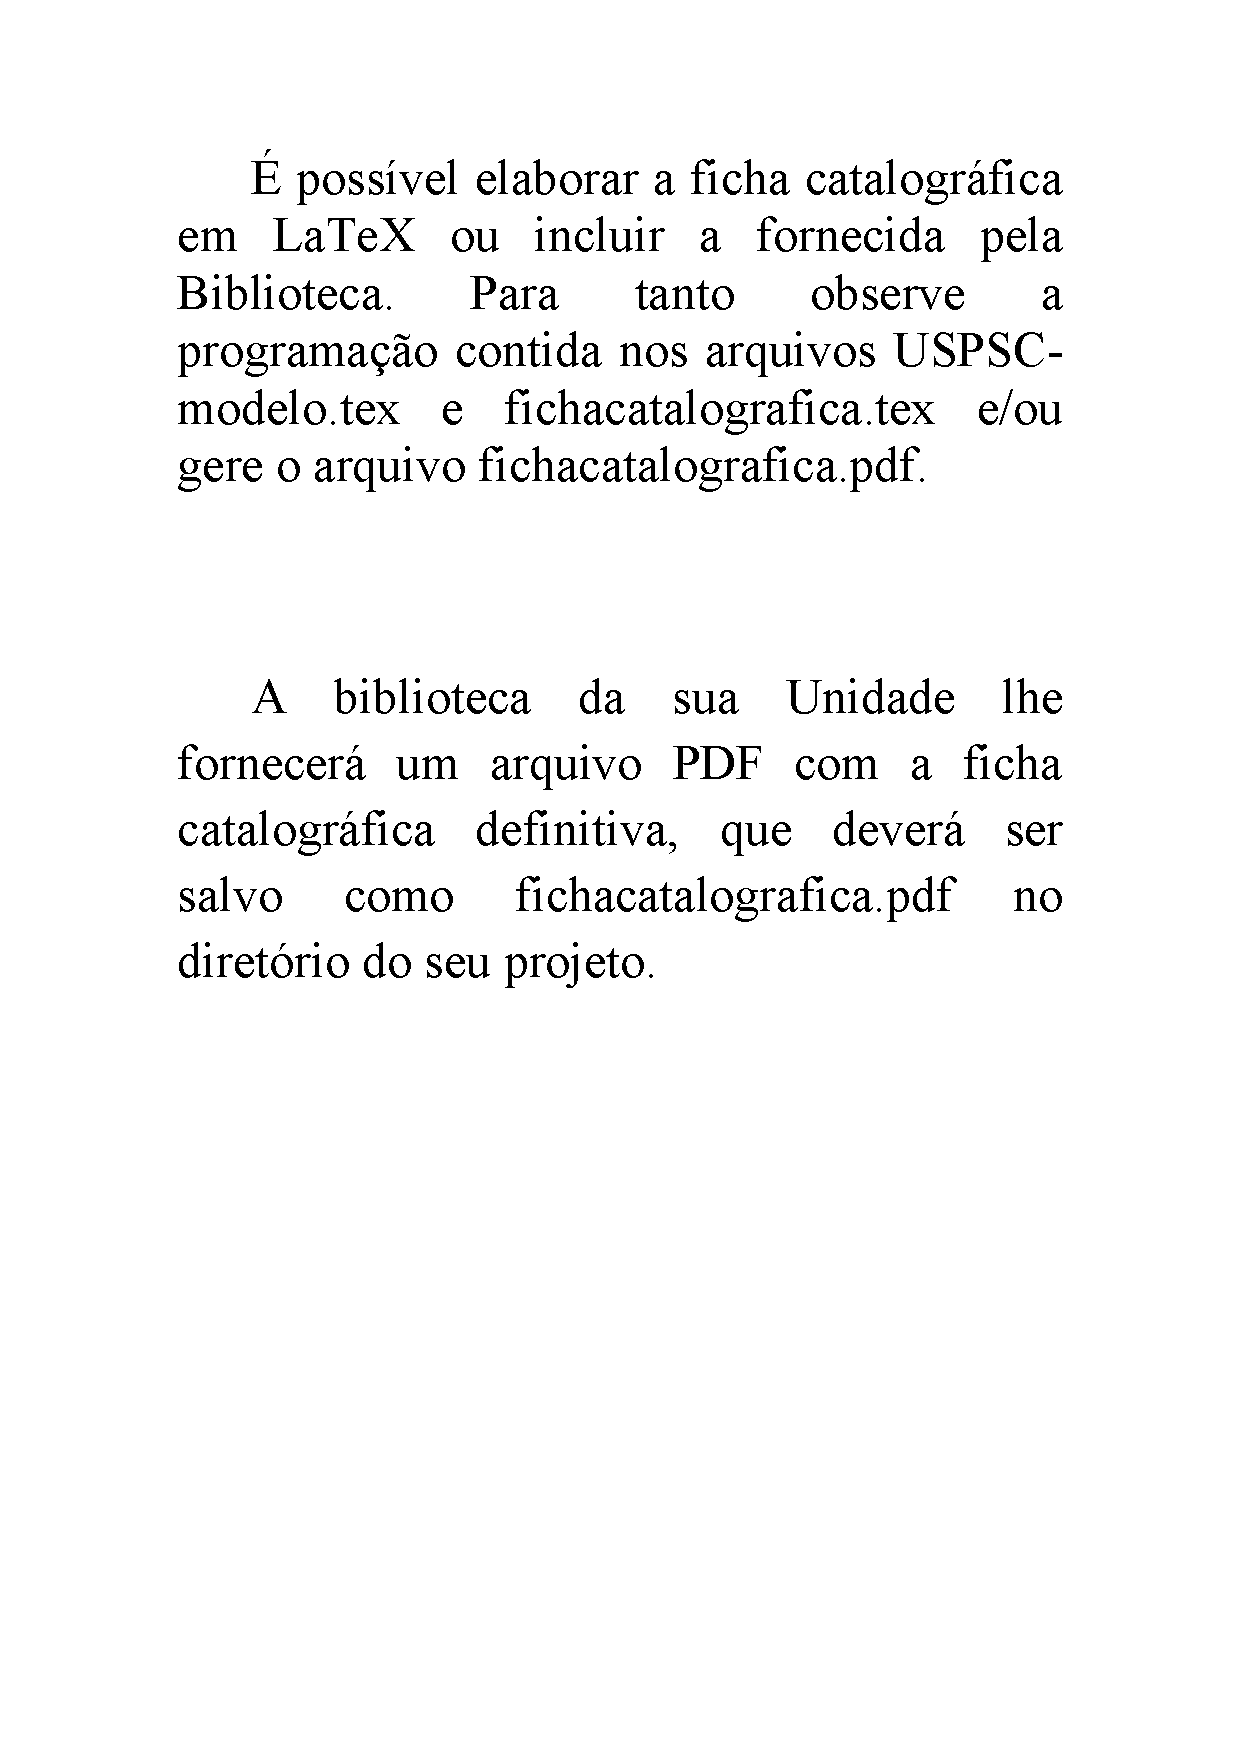
\includepdf{fichacatalografica.pdf}
%\end{fichacatalografica}

% Se você optar por elaborar a ficha catalográfica, deverá 
% incluir uma % antes das 3 linhas acima e tirar a % antes
% do comando % ---
% Inserir a ficha bibliografica
% ---
% Isto é um exemplo de Ficha Catalográfica, ou ``Dados internacionais de
% catalogação-na-publicação''. Você pode utilizar este modelo como referência. 
% Porém, provavelmente a biblioteca da sua universidade lhe fornecerá um PDF
% com a ficha catalográfica definitiva após a defesa do trabalho. Quando estiver
% com o documento, salve-o como PDF no diretório do seu projeto e substitua todo
% o conteúdo de implementação deste arquivo pelo comando abaixo:
%
\begin{fichacatalografica}
	\hspace{-1.4cm}
	\imprimirnotaautorizacao \\ \\
	%\sffamily
	\vspace*{\fill}					% Posição vertical
	\begin{center}					% Minipage Centralizado
		\imprimirnotabib \\
\begin{table}[htb]
	\scriptsize
	\centering	
	\begin{tabular}{|p{0.9cm} p{8.7cm}|}
		\hline
	      & \\
		  &	  \imprimirautorficha     \\
		
		 \imprimircutter & 
							\hspace{0.4cm}\imprimirtitulo~  / ~\imprimirautor~ ;  ~\imprimirorientadorcorpoficha. -- 	\imprimirlocal, \imprimirdata.   \\
		
		  &  % Para incluir nota referente à versão corrigida no corpo da ficha,
			  % incluir % no início da linha acima e tirar a % do início da linha abaixo
			  %	\hspace{0.4cm} \imprimirtitulo~  / ~\imprimirautor~ ; ~\imprimirorientadorcorpoficha~- ~\imprimirnotafolharosto. -- \imprimirlocal, \imprimirdata.  \\
		
			\hspace{0.4cm}\pageref{LastPage} p. : il. (algumas color.) ; 30 cm.\\ 
		  & \\
		  & 
		    \hspace{0.4cm}\imprimirnotaficha ~--~ 
						  \imprimirunidademin, 
						  \imprimiruniversidademin, 
		                  \imprimirdata. \\ 
		  & \\                 
		   % Para incluir nota referente à versão corrigida em notas,
		    % incluir uma % no início da linha acima e	
		    % tirar a % do início da linha abaixo
		    % & \hspace{0.4cm}\imprimirnotafolharosto \\ 
		  & \\ 
		  & \hspace{0.4cm}1. LaTeX. 2. abnTeX. 3. Classe USPSC. 4. Editoração de texto. 5. Normalização da documentação. 6. Tese. 7. Dissertação. 8. Documentos (elaboração). 9. Documentos eletrônicos. I. \imprimirorientadorficha. 
		   II. Título. \\
	
		     %Se houver co-orientador, inclua % antes da linha (antes de II. Título.) 
		     %          e tire a % antes do comando abaixo 
		     %III. Título. \\   
		  \hline
	\end{tabular}
\end{table}
	\end{center}
\end{fichacatalografica}
% ---


%% ---
% Inserir a ficha bibliografica
% ---
% Isto é um exemplo de Ficha Catalográfica, ou ``Dados internacionais de
% catalogação-na-publicação''. Você pode utilizar este modelo como referência. 
% Porém, provavelmente a biblioteca da sua universidade lhe fornecerá um PDF
% com a ficha catalográfica definitiva após a defesa do trabalho. Quando estiver
% com o documento, salve-o como PDF no diretório do seu projeto e substitua todo
% o conteúdo de implementação deste arquivo pelo comando abaixo:
%
\begin{fichacatalografica}
	\hspace{-1.4cm}
	\imprimirnotaautorizacao \\ \\
	%\sffamily
	\vspace*{\fill}					% Posição vertical
	\begin{center}					% Minipage Centralizado
		\imprimirnotabib \\
\begin{table}[htb]
	\scriptsize
	\centering	
	\begin{tabular}{|p{0.9cm} p{8.7cm}|}
		\hline
	      & \\
		  &	  \imprimirautorficha     \\
		
		 \imprimircutter & 
							\hspace{0.4cm}\imprimirtitulo~  / ~\imprimirautor~ ;  ~\imprimirorientadorcorpoficha. -- 	\imprimirlocal, \imprimirdata.   \\
		
		  &  % Para incluir nota referente à versão corrigida no corpo da ficha,
			  % incluir % no início da linha acima e tirar a % do início da linha abaixo
			  %	\hspace{0.4cm} \imprimirtitulo~  / ~\imprimirautor~ ; ~\imprimirorientadorcorpoficha~- ~\imprimirnotafolharosto. -- \imprimirlocal, \imprimirdata.  \\
		
			\hspace{0.4cm}\pageref{LastPage} p. : il. (algumas color.) ; 30 cm.\\ 
		  & \\
		  & 
		    \hspace{0.4cm}\imprimirnotaficha ~--~ 
						  \imprimirunidademin, 
						  \imprimiruniversidademin, 
		                  \imprimirdata. \\ 
		  & \\                 
		   % Para incluir nota referente à versão corrigida em notas,
		    % incluir uma % no início da linha acima e	
		    % tirar a % do início da linha abaixo
		    % & \hspace{0.4cm}\imprimirnotafolharosto \\ 
		  & \\ 
		  & \hspace{0.4cm}1. LaTeX. 2. abnTeX. 3. Classe USPSC. 4. Editoração de texto. 5. Normalização da documentação. 6. Tese. 7. Dissertação. 8. Documentos (elaboração). 9. Documentos eletrônicos. I. \imprimirorientadorficha. 
		   II. Título. \\
	
		     %Se houver co-orientador, inclua % antes da linha (antes de II. Título.) 
		     %          e tire a % antes do comando abaixo 
		     %III. Título. \\   
		  \hline
	\end{tabular}
\end{table}
	\end{center}
\end{fichacatalografica}
% ---


% As informações que compõem a ficha catalográfica estão 
% definidos no arquivo USPSC-pre-textual-UUUU.tex
% ---


% ---
% Inserir errata
% ---

%\begin{errata}
%	\OnehalfSpacing 			
%	A errata é um elemento opcional, que consiste de uma lista de erros da obra, precedidos pelas folhas e linhas onde eles ocorrem e seguidos pelas correções correspondentes. Deve ser inserida logo após a folha de rosto e conter a referência do trabalho para facilitar sua identificação, conforme a ABNT NBR 14724 \cite{nbr14724}.
%	
%	Modelo de Errata:
%		
%	\begin{flushleft} 
%			\setlength{\absparsep}{0pt} % ajusta o espaçamento da referência	
%			\SingleSpacing 
%			\imprimirautorabr~ ~\textbf{\imprimirtitulo}.	\imprimirdata. \pageref{LastPage}p. 
%			%Substitua p. por f. quando utilizar oneside em \documentclass
%			%\pageref{LastPage}f.
%			\imprimirtipotrabalho~-~\imprimirinstituicao, \imprimirlocal, \imprimirdata. 
% 	\end{flushleft}
%\vspace{\onelineskip}
%\OnehalfSpacing 
%\center
%\textbf{ERRATA}
%\vspace{\onelineskip}
%\OnehalfSpacing 
%\begin{table}[htb]
%	\center
%	\footnotesize
%	\begin{tabular}{p{1.4cm} p{1cm} p{3cm} p{3cm} }
%		\hline
%		\textbf{Folha} & \textbf{Linha}  & \textbf{Onde se lê}  & \textbf{Leia-se}  \\
%			\hline
%			1 & 10 & auto-conclavo & autoconclavo\\
%		\hline
%	\end{tabular}
%\end{table}
%
%
%\end{errata}
% ---

% ---
% Inserir folha de aprovação
% ---

% A Folha de aprovação é um elemento obrigatório da NBR 4724/2011 (seção 4.2.1.3). 
% Após a defesa/aprovação do trabalho, gere o arquivo folhadeaprovacao.pdf da página assinada pela banca 
% e iclua o arquivo utilizando o comando abaixo:
%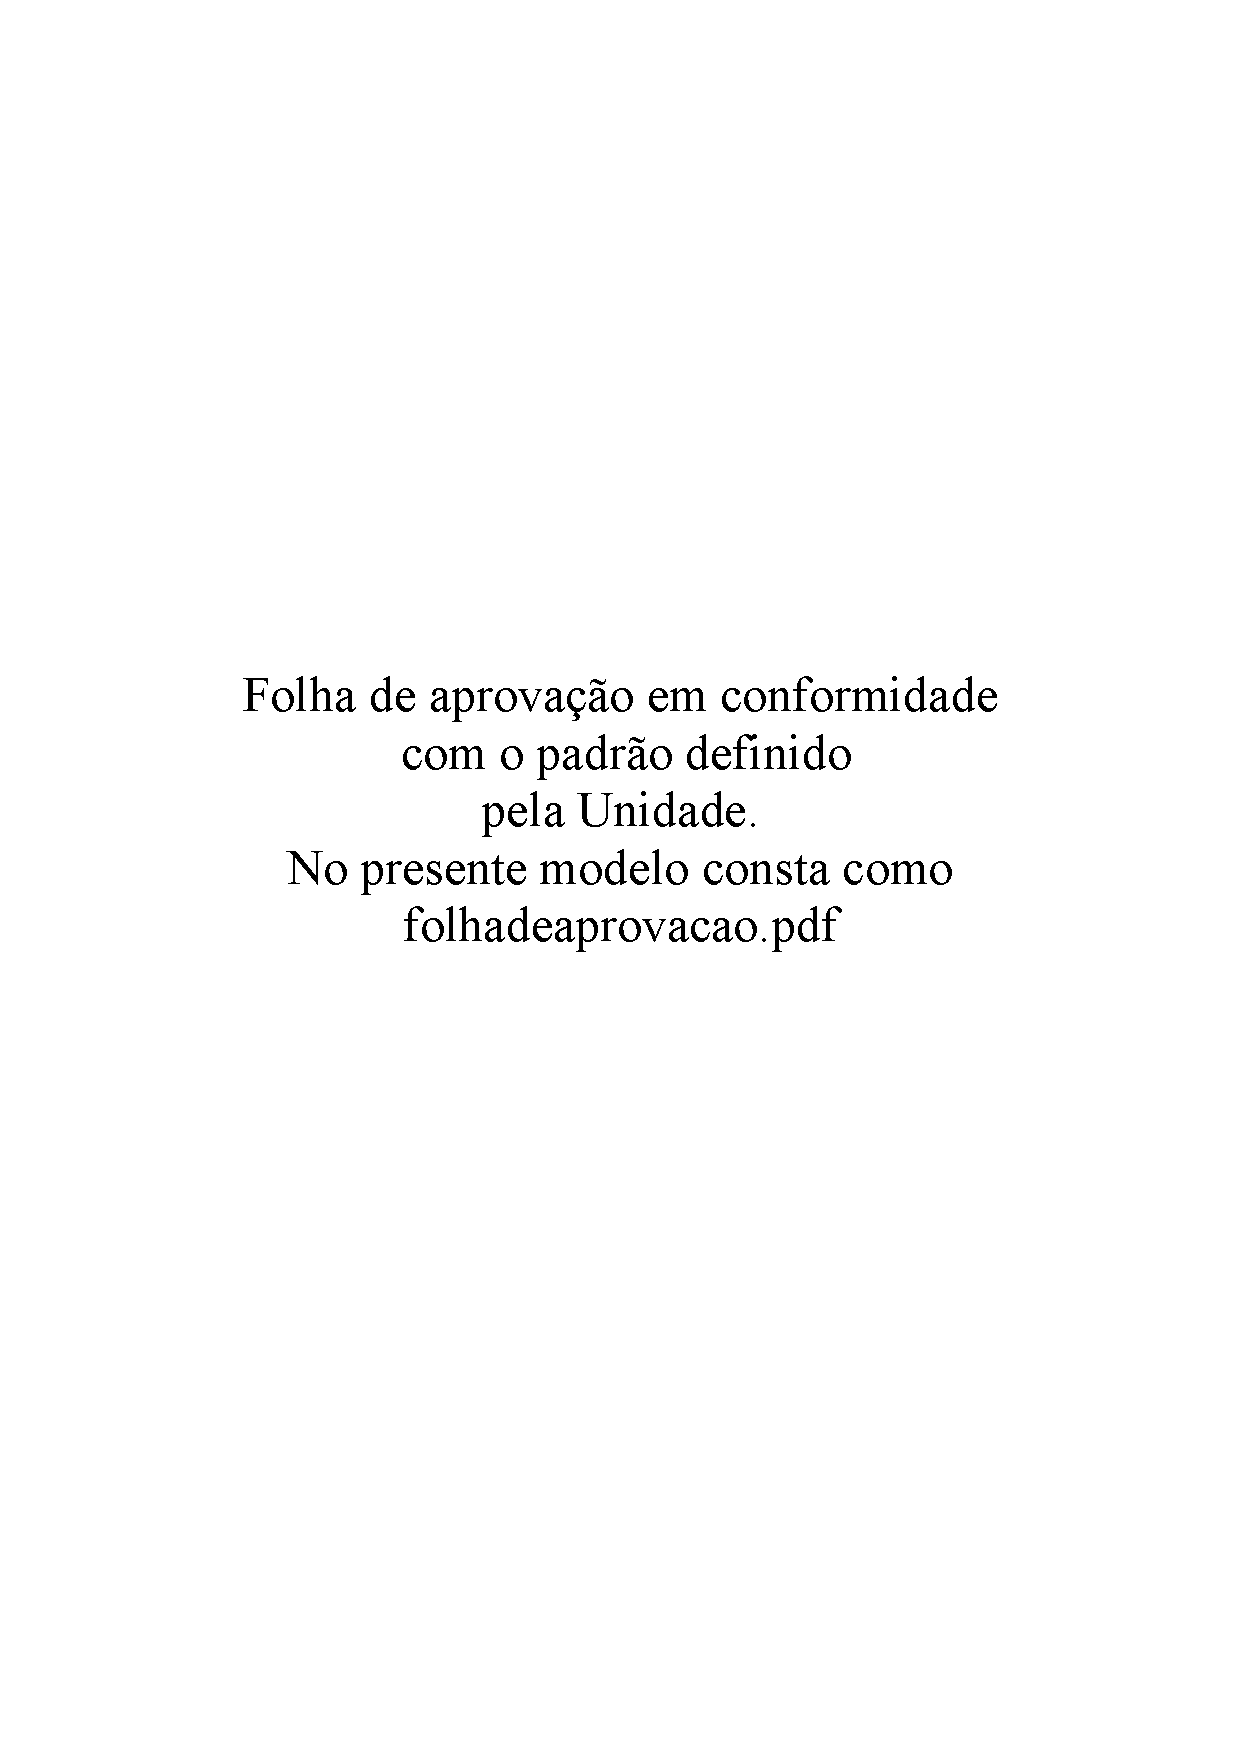
\includepdf{folhadeaprovacao.pdf}

% Alternativa para a Folha de Aprovação:
% Se for a sua opção elaborar uma folha de aprovação, insira uma % antes do comando acima que inclui o arquivo folhadeaprovacao.pdf,
% tire o % do comando abaixo e altere o arquivo folhadeaprovacao.tex conforme suas necessidades
%% Alternativa para a Folha de Aprova��o 
% Se esta for a sua op��o, exclua inclus�o feita acima do arquivo folhadeaprovacao.pdf
%
\begin{folhadeaprovacao}
  \begin{center}
       {\ABNTEXchapterfont\bfseries\large\imprimirautor}
	 \vspace*{2cm}
   
    \begin{center}
      \ABNTEXchapterfont\bfseries\Large\imprimirtitulo
    \end{center}
		\vspace*{2cm}
		\hspace{.45\textwidth}
    \begin{minipage}{.5\textwidth}
        \imprimirpreambulo
    \end{minipage}
		\vspace*{2cm}
    %\vspace*{\fill}
	\end{center}

  \begin{center}
	  {\ABNTEXchapterfont\bfseries\large\ {Data de defesa: 02 de outubro de 2015} \\}
		\vspace*{\fill}
	  {\ABNTEXchapterfont\bfseries\large\ {Comiss\~ao Julgadora:} \\}
		%Trabalho aprovado. \imprimirlocal, 2 de outubro de 2015:
		
		%\assinatura{\textbf{\imprimirorientador} \\ Orientador} 
		\assinatura{\textbf{\imprimirorientador} \\}
    % Se for ORIENTADOR, inclua % no in�cio do comando abaixo e tire a % do pr�ximo comando 
		\renewcommand{\orientadorname}{Orientadora}
		%\renewcommand{\orientadorname}{Orientador}

		\imprimirorientadorRotulo
		\par
		\assinatura{\textbf{Professor} \\ Convidado1}
	
		\assinatura{\textbf{Professor} \\ Convidado2}
		%\assinatura{\textbf{Professor} \\ Convidado3}
		%\assinatura{\textbf{Professor} \\ Convidado4}
		%\begin{center}
		\vspace*{\fill}
   	{\ABNTEXchapterfont\bfseries\large\imprimirlocal}
    \par
    {\ABNTEXchapterfont\bfseries\large\imprimirdata}
\end{center}
\end{folhadeaprovacao}
% ---

%
\includepdf{PaginaEmBranco.pdf}

% ---
% Dedicatória
% ---
%\begin{dedicatoria}
%   \vspace*{\fill}
%   \centering
%   \noindent
%   \textit{ Este trabalho é dedicado aos alunos da USP, como uma contribuição\\
%  das Bibliotecas do Campus USP de São Carlos para o desenvolvimento\\
%	e disseminação da pesquisa científica da Universidade.} \vspace*{\fill}
%\end{dedicatoria}
% ---

% ---
% Agradecimentos
% ---=====
%\begin{agradecimentos}
%A motivação para o desenvolvimento da classe USPSC e dos modelos de dissertações e teses foi decorrente de solicitações de usuários das Bibliotecas do Campus USP de São Carlos. 
%
%O Grupo desenvolvedor do Pacote USPSC, atualmente composto da Classe USPSC e do  Modelo para teses e dissertações em \LaTeX\ utilizando a classe USPSC, agradece especialmente ao Luis Olmes, doutorando do Instituto de Ciências Matemáticas e de Computação (ICMC) da Universidade de São Paulo (USP), pelas primeiras orientações sobre o \LaTeX\ .
%
%Agradecemos ao Lauro César Araujo pelo desenvolvimento da classe  \abnTeX, modelos canônicos e tantas outras contribuições que nos permitiu o desenvolvimento da classe USPSC e seus modelos.
%
%Os nossos agradecimentos aos integrantes do primeiro projeto abn\TeX\, Gerald Weber, Miguel Frasson, Leslie H. Watter, Bruno Parente Lima, Flávio de Vasconcellos Corrêa, Otavio Real Salvador, Renato Machnievscz, e a todos que contribuíram para que a produção de trabalhos acadêmicos em conformidade com as normas ABNT com \LaTeX\ fosse possível.
%
%Agradecemos ao grupo de usuários
%\emph{latex-br}{\url{http://groups.google.com/group/latex-br}}, aos integrantes do grupo
%\emph{\abnTeX}{\url{http://groups.google.com/group/abntex2}  e \url{http://www.abntex.net.br/}}~que contribuem para a evolução do \abnTeX.
%\end{agradecimentos}
% ---

% ---
% Epígrafe
% ---
%\begin{epigrafe}
%    \vspace*{\fill}
%	\begin{flushright}
%		\textit{``O estudo, a busca da verdade e da beleza são domínios \\
%		em que nos é consentido sermos crianças por toda a vida.''\\
%		Albert Einstein}
%	\end{flushright}
%\end{epigrafe}
% ---

% A T E N Ç Ã O
% Se o idioma do texto for em inglês, o abstract deve preceder o resumo
% resumo em português
%

% Abstract
% ---
%% Abstract.tex
% ---
% Abstract
% ---
\autor{Silva, M. J.}
\begin{resumo}[Abstract]
 \begin{otherlanguage*}{english}
	\begin{flushleft} 
		\setlength{\absparsep}{0pt} % ajusta o espaçamento dos parágrafos do resumo		
 		\SingleSpacing 
 		\imprimirautorabr~ ~\textbf{\imprimirtitleabstract}.	\imprimirdata.  \pageref{LastPage}p. 
		%Substitua p. por f. quando utilizar oneside em \documentclass
		%\pageref{LastPage}f.
		\imprimirtipotrabalho~-~\imprimirinstituicao, \imprimirlocal, 	\imprimirdata. 
 	\end{flushleft}
\OnehalfSpacing
This project proposes the development of a software for non-linear system's model identification, focusing on wind power plants. The chosen model  for wind power plants is well-known in the literature and is capable of representing the most common wind turbine type during both steady-state and transients. The method applied to identify the model is composed of two optimization algorithms. At the begining of the process, an heuristic approach based on Mean-Variance Mapping Optimization is used in order to reduce the parameter's search region around a possible solution. Afterward, a non-linear algorithm based on Trajectory Sensitivity is used to fine-tune the parameters. The method validation will be made using data from simulated systems. Also, a guided user interface will be developed for this application, aiding new users. All coding for this project will be made in Python.


\textbf{Keywords}: Model identification. Wind power plants. MVMO. Trajectory sensitivity. Python.
 \end{otherlanguage*}
\end{resumo}


% Resumo
% ---
%% Resumo.tex
% ---
% Resumo
% ---
\setlength{\absparsep}{18pt} % ajusta o espaçamento dos parágrafos do resumo		

\begin{resumo}[Resumo]

\begin{otherlanguage*}{brazil}

\begin{flushleft} 
	\setlength{\absparsep}{0pt} % ajusta o espaçamento da referência	
	\SingleSpacing 
	\imprimirautorabr~ ~\textbf{\imprimirtitulo}.	\imprimirdata. \pageref{LastPage}p. 
	%Substitua p. por f. quando utilizar oneside em \documentclass
	%\pageref{LastPage}f.
	\imprimirtipotrabalho~-~\imprimirinstituicao, \imprimirlocal, \imprimirdata. 
\end{flushleft}

\OnehalfSpacing 			

O presente trabalho prop\~oe o desenvovlimento de um \textit{software} voltado para a identifica\c{c}\~ao de modelos de sistemas n\~ao-lineares, com enfoque em plantas e\'olicas. O modelo escolhido para plantas e\'olicas \'e bem consolidado na literatura, sendo capaz de representar o comportamento de geradores mais utilizados nas instala\c{c}\~oes deste tipo tanto durante o regime permanente quanto em transit\'orios. O m\'etodo utilizado para a identifica\c{c}\~ao do modelo \'e constitu\'ido por dois algoritmos de otimiza\c{c}\~ao. Primeiramente, \'e empregada uma abordagem heur\'istica, baseada em Otimiza\c{c}\~ao por Mapeamento de M\'edia-Vari\^ancia, a fim de reduzir a regi\~ao de busca dos par\^ametros em torno de uma poss\'ivel solu\c{c}\~ao. Em seguida, lan\c{c}a-se m\~ao de um algoritmo n\~ao-linear, baseado no M\'etodo de Sensibilidade de Trajet\'oria, para realizar os ajustes finais nos valores dos par\^ametros. A valida\c{c}\~ao do m\'etodo ser\'a feita utilizando medidas de sistemas simulados. Com o intuito de facilitar a experi\^encia do usu\'ario com o programa, ser\'a desenvolvida uma interface gr\'afica para o \textit{software}. Tanto as rotinas para identifica\c{c}\~ao de modelos quanto a interface gr\'afica ser\~ao desenvolvidas em Python.
 

\textbf{Palavras-chave}: Identifica\c{c}\~ao de modelos. Plantas e\'olicas. MVMO. Sensibilidade de trajet\'oria. Python.

\end{otherlanguage*}

\end{resumo}
% ---

% ---
% inserir lista de ilustrações
% ---
\pdfbookmark[0]{\listfigurename}{lof}
\listoffigures*
\cleardoublepage
% ---

% ---
% inserir lista de tabelas
% ---
\pdfbookmark[0]{\listtablename}{lot}
\listoftables*
\cleardoublepage
% ---

% ---
% inserir lista de quadros
% ---
%\pdfbookmark[0]{\listofquadroname}{loq}
%\listofquadro*
%\cleardoublepage
% ---

% ---
% inserir lista de abreviaturas e siglas
% ---
\begin{siglas}
    \item[ABEE\'olica] Brazilian Wind Energy Association
    \item[ANEEL] Brazilian Electricity Regulatory Agency
    \item[DFIG] Doubly Fed Induction Generator
    \item[EESG] Electrical Excited Synchronous Generator
    \item[EU] European Union
    \item[GUI] Graphical User Interface
	\item[IEEE] Institute of Electrical and Electronics Engineers
	\item[LSC] Line-Side Converter
	\item[MVMO] Mean-Variance Mapping Optimization
	\item[PMU] Phasor Measurement Unit
	\item[PMSG] Permanent Magnet Synchronous Generator
    \item[PROINFA] Program of Incentive to Alternative Electric Energy Sources
    \item[RoW] Rest of World
    \item[RSC] Rotor-Side Converter
    \item[SCIG] Squirrel Cage Induction Generator
    \item[TSM] Trajectory Sensitivity Method
    \item[US] United States of America
    \item[UK] United Kingdom
    \item[WECC] Western Electricity Coordinating Council
    \item[WPP] Wind Power Plant
    \item[WRIG] Wound Rotor Induction Generator
    \item[WTG] Wind Turbine Generator

	
\end{siglas}
% ---

% ---
% inserir lista de símbolos
% ---
\begin{simbolos}
	\item[$e$] Error vector
	\item[$f_{s}$] MVMO scaling factor
	\item[$G$] Error sensibility
	\item[$h$] MVMO transformation function
	\item[$i_{max}$] Maximum generator current
	\item[$J$] $l^{2}$-norm of error vector
	\item[$k_{I}$]	Gain of PI controller
	\item[$k_{VC}$] Gain of proportional block
	\item[$p$] Parameter vector
	\item[$p_{i}$] i-th element of the parameter vector
	\item[$\bar{p_{i}}$] Mean value of i-th element of the parameter vector
	\item[$P$] Active power generated
	\item[$Q$] Reactive power generated
	\item[$R$] Thevenin equivalent resistance
	\item[$s_{i}$] MVMO shape factor of i-th parameter
	\item[$T_{I}$] Time constant of PI controller
	\item[$T_{V}$] Time constant of delay block
	\item[$u$] Input vector
	\item[$v^{*}$] Bus voltage threshold
	\item[$v_{d}$] Direct-axis voltage component
	\item[$v_{i}$] Variance of i-th parameter
	\item[$v_{q}$] Quadrature-axis voltage component
	\item[$v_{T}$] Bus voltage magnitude
	\item[$x$] State vector
	\item[$X$] Thevenin equivalent reactance
	\item[$y$] Output vector
	\item[$y_{r}$] Output measured on real system
	\item[$\phi_{v}$] Bus voltage angle
	\item[$\Gamma$] Jacobian matrix of error sensibility
\end{simbolos}
% ---
% ---
% inserir o sumario
% ---
\pdfbookmark[0]{\contentsname}{toc}
\tableofcontents*
\cleardoublepage
% ---
% ----------------------------------------------------------
% ELEMENTOS TEXTUAIS
% ----------------------------------------------------------
\textual
% Os capítulos são inseridos como arquivos externos 

% ---
% Capítulo 1 - Introdução
% ---
\chapter[Introduction]{Introduction}
\label{ch: Intro}

During the last two decades, the world has seen an increasing participation of renewable sources in power generation, leaded mainly by wind and solar energy. These technologies provide an alternative to sources based on fossil fuel, such as oil, gas and coal, lowering pollution levels and reducing greenhouse gas emissions. On the other hand, the power output from these sources strongly relies on weather conditions and cannot be fully controlled.

This increase is seen worldwide, as part of policies to reduce the human impact on climate and the environment. This `renewable wave' is leaded mainly by European countries, specially in the European Union (EU), United States (US) and China. In particular, the EU has set in 2010 a strategy plan to reduce its greenhouse emissions by at least 20\% compared to 1990 levels and increase the share of renewable sources to at least 20\% by 2020 \cite{Europe2020}.

Brazil does not lag far behind the EU regarding renewable sources policies. In 2002, the country passed a bill that, among other actions, creates the Program of Incentive to Alternative Electric Energy Sources (PROINFA). This program aims to increase the share of wind, solar, small hydro and biomass energy production. The final goal is to have these energy sources corresponding to 10\% of Brazil's annual energy consumption by 2024 \cite{Brazil2002}.

\section{Wind Energy}

Those policies promoted the increase of wind energy participation, reaching a scenario where it is one of the main energy sources of some countries, such as Denmark and Ireland. In the EU, wind energy alone generated 417 TWh in 2019, covering 15\% of the electricity demand, a share 1\% higher than 2018, with wind turbine generators (WTGs) installed both onshore (within the countries) and offshore (in the ocean). Among the EU countries, Denmark leads in this sector, with 48\% of its demand supplied by wind power plants (WPPs), followed by Ireland (33\%), Portugal (27\%) and Germany (26\%). The total installed capacity across the 28 EU countries (UK included) is 192 GW, with Germany in first position, with a total installed capacity of 61 GW, followed by Spain and the United Kingdom (UK), with 26 and 24 GW installed, respectively \cite{WindEurope2020}. Figure \ref{fig: EUrank} displays the detailed percentage of electricity demand covered by wind in the EU.

\begin{figure}[h]
	\caption{Share of electricity demand in the EU covered by wind energy during 2019}
	\begin{center}
		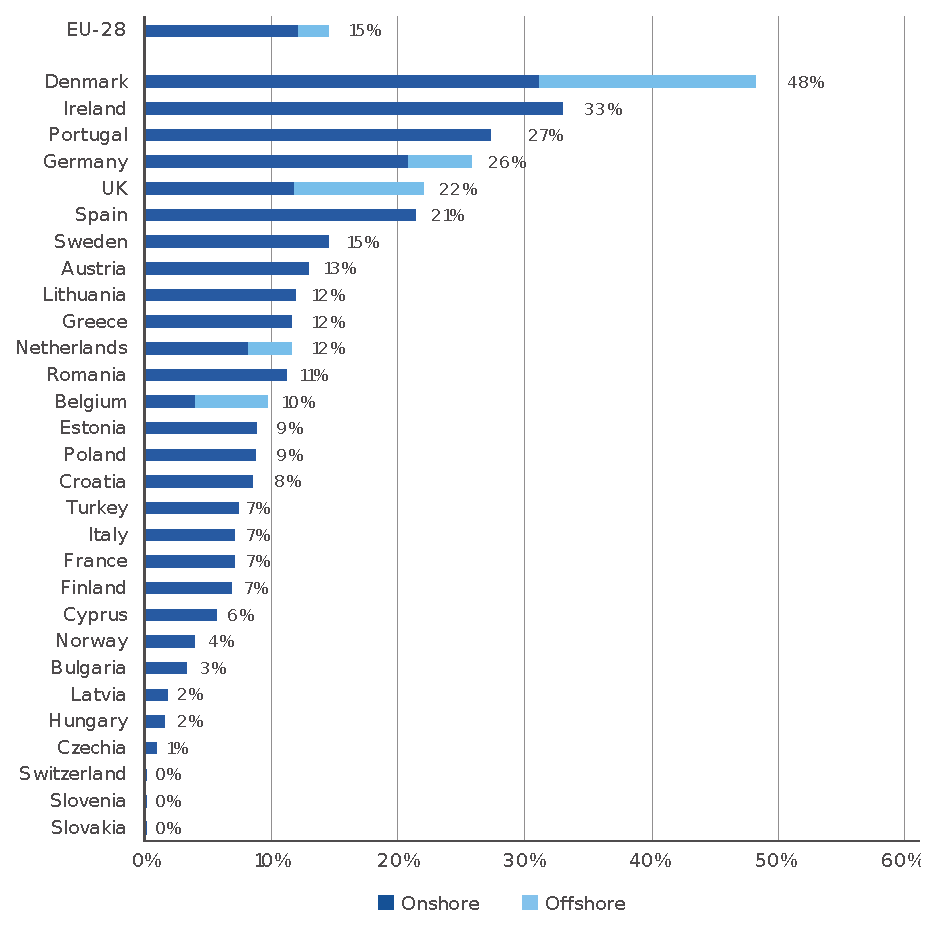
\includegraphics[scale=0.65]{Images/EUrank2019.eps}
	\end{center}
	\label{fig: EUrank}
	\legend{Source: Wind Europe, 2020}
\end{figure}

In Brazil, wind energy contributed to the electricity matrix with 48.5 TWh during 2018, resulting in a participation share of 8.1\%. For comparison, Itaipu, the largest power plant in Brazil, has produced 96.5 TWh during the same period. But, while other sources, such as gas and coal, had their share lowered, wind energy had the highest increase among sources comparing to 2017, increasing its contribution by 14.4\% \cite{EPE2019}.

Regarding the installed capacity, wind power plants appear in \nth{2} place, with 15.5 GW installed, only behind hydro power plants \cite{ABEEolica2020}, as shown in Figure \ref{fig: BRshare}. However, there is still plenty of energy yield for this source to be explored. In \cite{Atlas2001} is shown that Brazil has potential to generate 272.2 TWh per year, with an installed capacity of 143.5 GW. The Northeast Region has the higher potential, with an annual energy yield of 144.3 TWh and potential to host up to 75.0 GW. Also, the wind regime in the Northeast Region is complimentary to the water regime of the main river responsible to power generation in the region, as presented by Figure \ref{fig: WindWater}. This characteristic would help controlling reservoir water level during dry season, an important resource not only for power generation, but also irrigation of crops and water supply \cite{ANEEL2005}.

\begin{figure}[ht]
	\caption{Electricity generation in Brazil by source during 2019}
	\begin{center}
		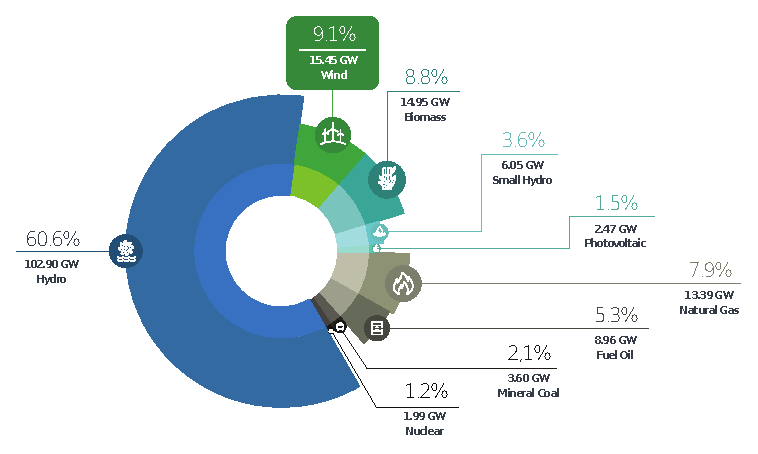
\includegraphics[scale=1]{Images/BRshare20.eps}
	\end{center}
	\label{fig: BRshare}
	\legend{Source: ABEE\'olica, 2020}
\end{figure}

\begin{figure}[hb]
	\caption{Wind and water regime in the Brazilian Northeast Region}
	\begin{center}
		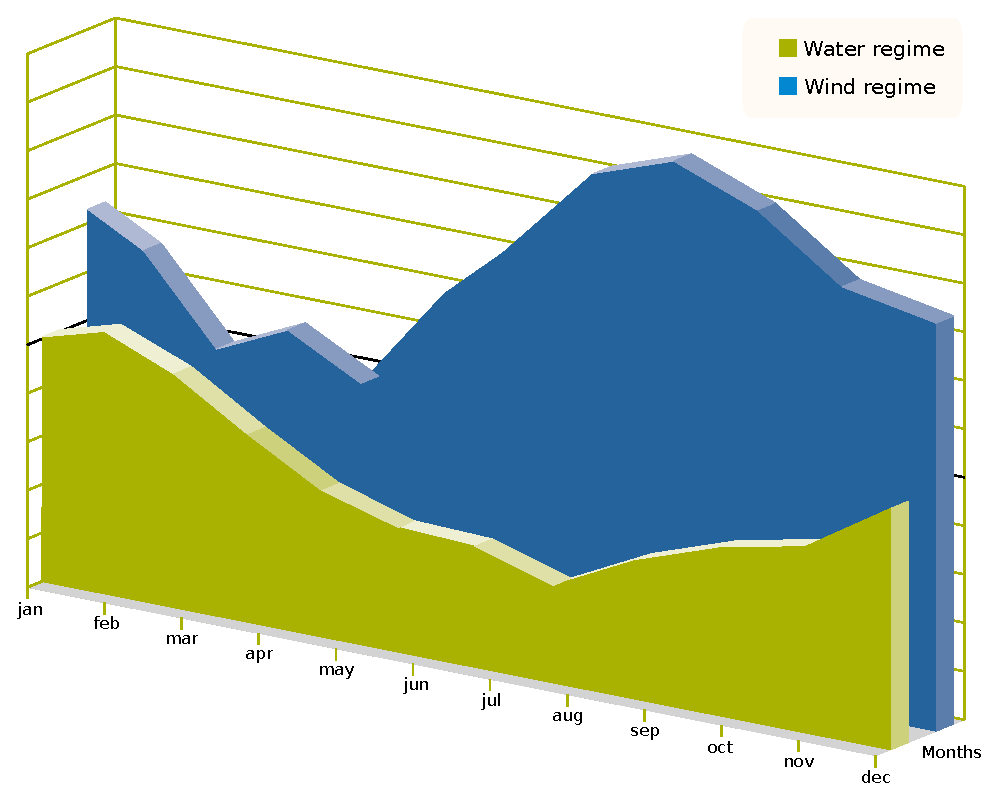
\includegraphics[scale=0.5]{Images/WindWater.eps}
	\end{center}
	\label{fig: WindWater}
	\legend{Source: ANEEL, 2005}
\end{figure}

Therefore, it is expected that wind energy will increase its participation in electricity generation in the near future. However, some aspects of the wind energy must be considered prior to the implementation of wind power plants on large scale.

The main difficulties are due to the nature of the energy source and characteristics of the generator. The wind regime is not constant and evenly distributed across the country, depending on the region geography and vegetation. This results in a energy source that is not entirely reliable and concentrated on a certain area. Wind turbine generators are usually partially or entirely decoupled from the grid via power electronic converters, resulting in machines with low inertia. Thus, the system may experience stability problems during transients due to the high penetration of these machines \cite{Xiong2019}.

In order to maintain the electrical power system reliable, studies simulating various conditions must be performed beforehand, so the operators can be prepared for different fault scenarios. Therefore, robust mathematical models, capable of adequately simulate the behaviour of every component on the grid, are vital to these studies. Otherwise, operators will not be able to solve the fault problem or even provide a solution that will aggravate the fault.

\section{Difficulties in Representing Wind Power Plants}

With a growing share of energy covered by wind, system operators must consider how wind turbines affect the system stability during faults and maneuvers. To reach this goal, mathematical models capable of describing the behaviour of these machines are crucial. 

Obtaining these models, on the other hand, is not an easy task. Due to confidentiality, most manufacturers provide little or no information about the functioning of their wind turbine generators. In addition, there is a great amount of WTGs available, with different manufacturers, technologies, sizes and characteristics. Thus, a model that well describes a particular machine will not necessarily work for others.

Modelling entire wind power plants is even harder, since these facilities contain a large variety of WTGs spread over a wide area. Besides, line impedance of each generator is different, since their distances to the substation is not the same, as depicted in Figure \ref{fig: WPP}. Hence, having one model for every wind turbine within a power plant would result in a mathematical model with high computational cost and extremely complex \cite{Erlich2012}.

\begin{figure}[h]
	\caption{Example of Wind Power Plant}
	\begin{center}
		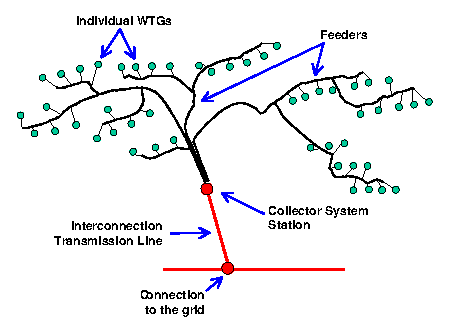
\includegraphics[scale=1.25]{Images/WPP.eps}
	\end{center}
	\label{fig: WPP}
	\legend{Source: Adapted from \cite{Muljadi2008}}
\end{figure}

In order to avoid using such complex models, many studies addressed the application of generic equivalent models to simulate the behaviour of WPPs. In particular, \cite{Ellis2011} shows that most wind power plants can be represented by a single-machine equivalent model. The benefits of using such equivalent model include reduction on model complexity and the fact it can be adjusted to match any given wind power plant. On the downside, these models cannot reproduce how particularities of each generator, such as wind speed and low voltage ride through capability, affects the WPP behaviour.

\section{Research Goals}

The main goal of this research is to develop a software for parameter estimation of nonlinear model and apply it to a wind power plant equivalent model used in transient stability studies. In order to achieve this goal, a hybrid estimation approach was applied combining two methods: Mean-Variance Mapping Optimization, a population-based metaheuristic approach, and Trajectory Sensitivity Method, a nonlinear approach. Also, as a secondary goal, a graphical user interface (GUI) was developed, so other users can easily apply the tool created. This research is a extension of \cite{Cari2015}, that focused on the parameter estimation using only Trajectory Sensitivity Method.

\section{Work Organization}

This section summarizes how the remainder of the text is organized. Chapter \ref{ch: Models} will focus on the generic models for wind turbine generators and power plants and the selected mathematical model for parameter estimation purposes will be presented. The hybrid estimation process proposed and its methods will be subject of chapter \ref{ch: Estimation}. The python package and GUI created in this research will be detailed on chapter \ref{ch: Software}. On chapter \ref{ch: Results}, the results obtained on this research will be discussed. Finally, chapter \ref{ch: Future} covers the future perspectives of this study.
% ---
% Capítulo 2 - Modelling of Wind Turbine Generators
% ---
\chapter{Modelling of Wind Turbine Generators}
\label{ch: Models}

Due to huge variety of wind turbine generators and their different characteristics, modelling each machine of a wind power plant separately would be a long and exhaustive work. To address this problem, studies such as \cite{Muljadi2008}, \cite{Ellis2011}, \cite{council2008wecc} and \cite{Asmine2011}, conducted specially by the Institute of Electrical and Electronics Engineers (IEEE) and the Western Electricity Coordinating Council (WECC), developed generic models able to predict the behaviour of entire wind power plants. Such models reduced the problem complexity, since they were composed of a single equivalent generator. A two-machine model is needed only in rare cases, such as when the wind power plant is composed of two or more types of wind turbines \cite{Ellis2011}.

\section{Generic Models of Wind Turbine Generators}

The studies mentioned above have concluded that commercial wind turbine generators could be sorted into four basic types, according to their characteristics and technologies \cite{Ellis2011}. These types are described in the following subsections.

\subsection{Type-1: Squirrel Cage Induction Generator (SCIG)}

The first type of wind turbine generator is composed of a Squirrel Cage Induction Generator (SCIG) connected to a wind turbine through a controlled gearbox, as displayed in Figure \ref{fig: WTG1}.

\begin{figure}[h]
	\caption{Representation of Type-1 Wind Turbine Generator}
	\begin{center}
		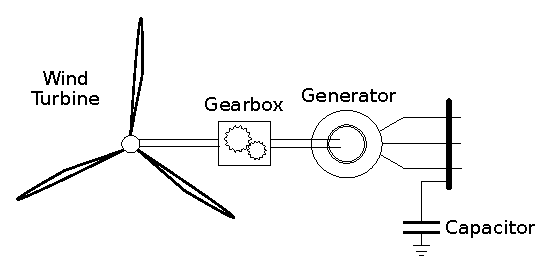
\includegraphics[scale=.8]{Images/Type1WTG.eps}
	\end{center}
	\label{fig: WTG1}
\end{figure}

Due to its torque-speed characteristics, generators of this type operate at constant rotor speed, requiring robust controllers on gearbox and blade. Besides, as usual to any induction generator, the SCIG absorbs reactive power during operation. Thus, capacitors are often employed for power factor correction purposes. Moreover, type-1 generators limit aerodynamic power by varying the pitch angle of their blades, imposing great mechanical stress on blades, shafts and gears, demanding a robust mechanical design and preventing these generators to operate above certain wind speed \cite{Ellis2011}. 

\subsection{Type-2: Wound Rotor Induction Generator (WRIG)}

Similarly to Type-1 WTG, Type-2 Wind Turbine Generators are composed of an asynchronous machine connected to a wind turbine via gearbox. However, instead of SCIG, Wound Rotor Induction Generator (WRIG) are used to convert kinetic energy into electricity. Generators of this type grant access to the rotor windings, allowing variances on the rotor resistance. As a direct consequence, this machine can operate in different wind speeds by adjusting its torque-speed curve as needed \cite{Ellis2011}. Therefore, Type-2 WTG have a WRIG with a variable resistance connected to its rotor terminals, as shown in Figure \ref{fig: WTG2}.

\begin{figure}[h]
	\caption{Representation of Type-2 Wind Turbine Generator}
	\begin{center}
		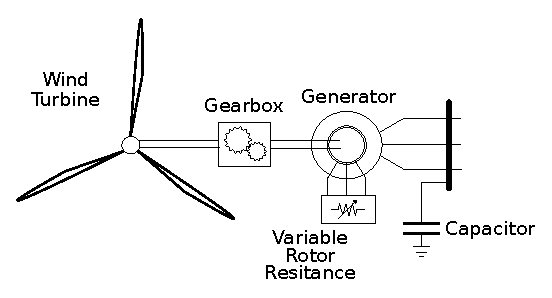
\includegraphics[scale=.8]{Images/Type2WTG.eps}
	\end{center}
	\label{fig: WTG2}
\end{figure}

Thus, this type of generator has three speed control systems, with rotor resistance control responding to rapid changes in speed, gearbox control for medium variations and pitch control for slow changes. These control systems work together to maintain power output at the desired level and reduce mechanical stress on components. The effects on the torque-speed curve caused by different rotor resistances are shown in Figure \ref{fig: Tw}.

\begin{figure}[h]
	\caption{Torque-speed curve}
	\begin{center}
		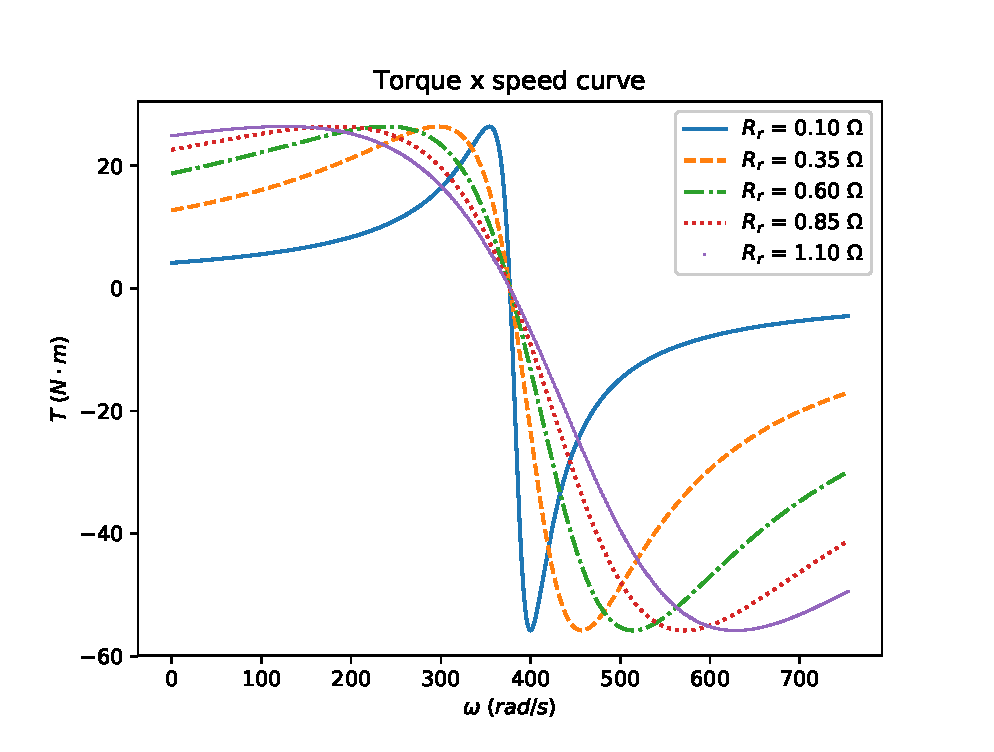
\includegraphics[scale=.6]{Images/Tw_curve.eps}
	\end{center}
	\label{fig: Tw}
\end{figure}

For a fixed power, increasing rotor resistance increases the speed needed on the shaft, allowing the wind turbine to operate above rated wind speed. However, the speed range is only $\pm 10\%$ of rated slip. Also, this machine still needs a reactive compensation circuit on its terminals, since it naturally drains reactive power from the grid \cite{Muljadi2010}.

\subsection{Type-3: Doubly Fed Induction Generator (DFIG)}

A Type-3 Wind Turbine Generator, often called Doubly Fed Induction Generator (DFIG), is also composed of a wound rotor machine connected to a wind turbine. But, instead of having a variable resistance connected to its rotor terminals, as the previous WTG type, DFIGs have their rotor windings supplied with AC voltage by a back-to-back frequency converter, as displayed in Figure \ref{fig: WTG3}. 

\begin{figure}[h]
	\caption{Representation of Type-3 Wind Turbine Generator}
	\begin{center}
		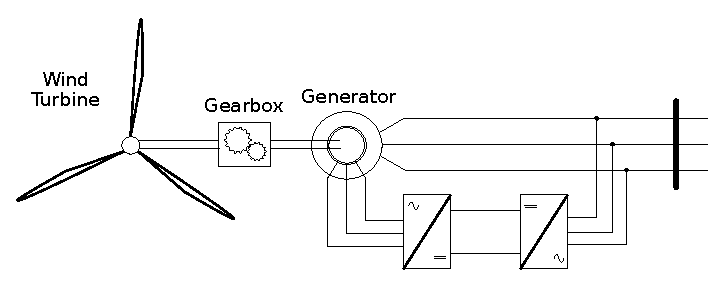
\includegraphics[scale=.8]{Images/Type3WTG.eps}
	\end{center}
	\label{fig: WTG3}
\end{figure}

The line-side converter (LSC) main purpose is to maintain voltage level on the DC link and provide reactive current during fault, while the rotor-side converter (RSC) controls active and reactive power generated by the machine by emulating different voltage frequencies on the rotor windings. By varying voltage frequency on the rotor circuit, this type of generator is able to supply power to the grid in a wider range of wind speed, reaching $\pm 30\%$ of rated slip. In addition, as result of the independent control of active and reactive power, reactive compensator circuits are no longer needed\cite{Muljadi2010}.

Since approximately $30\%$ of rated power flows through the rotor windings, power electronics components have lower specifications and do not have great impact on overall costs. On the other hand, these generators need regular maintenance due to slip rings, brushes and gearbox, preventing its broad use in offshore applications \cite{Yaramasu2015}.

\subsection{Type-4: Full-Converter Generator}

The last type of wind turbine generator, also called Full-Converter Generator, is composed of an electrical machine connected to the grid through a back-to-back frequency converter. The converters operate by controlling the frequency of the generated voltage so it matches the grid standard frequency. In this configuration, WTGs are able to produce energy in a large range of wind speed (up to almost 100\% of rated slip). Also, the connection between rotor and wind turbine shaft can be made directly or via gearbox. Likewise, it allows the use of both synchronous and asynchronous electrical machines as generator, with Permanent Magnet Synchronous Generator (PMSG), Electrical Excited Synchronous Generator (EESG) and SCIG being the most common, due to cost and maintenance purposes. Similar to DFIG, full-converter generators are able to independently control real and reactive power injected into or drained from the grid. However, since the entire generated power must flow through the power electronic devices, the overall cost of these generators is usually higher than other WTG types \cite{Yaramasu2015}. Figure \ref{fig: WTG4} depicts a typical Type-4 Wind Turbine Generator.

\begin{figure}[h]
	\caption{Representation of Type-4 Wind Turbine Generator}
	\begin{center}
		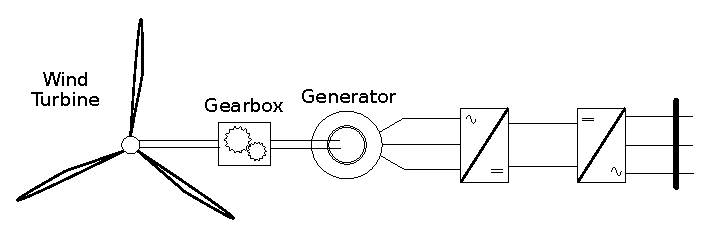
\includegraphics[scale=.8]{Images/Type4WTG.eps}
	\end{center}
	\label{fig: WTG4}
\end{figure}

Figure \ref{fig: WindShare} shows the evolution of share in installed capacity onshore for each generator type. The data shows how SCIG and WRIG lost space in the segment and how participation of DFIG and Full-Converter Generators rose, dominating the global market \cite{Magagna2017}.

\begin{figure}[h]
	\caption{Share of installed capacity for each wind turbine generator type}
	\begin{center}
		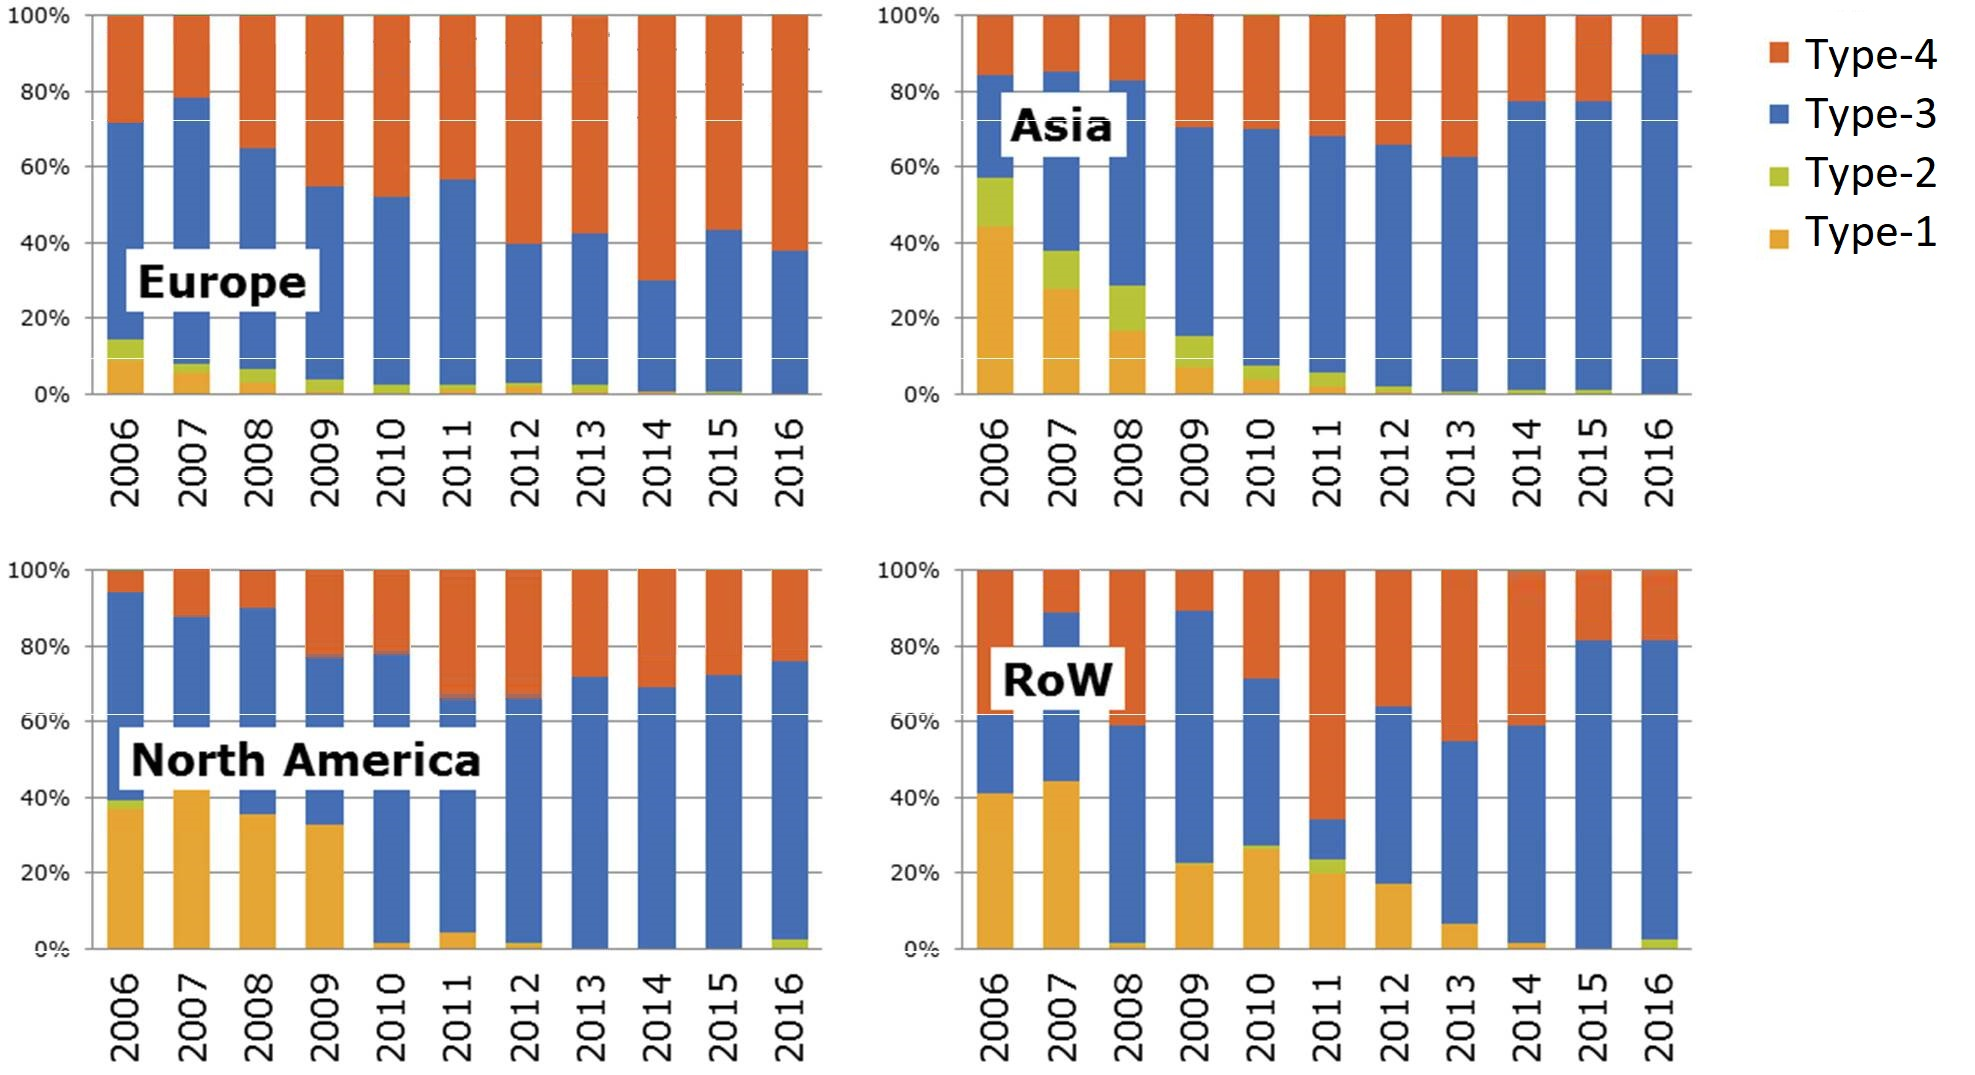
\includegraphics[scale=.2]{Images/WTGTypes.jpg}
	\end{center}
	\legend{Source: Adapted from \cite{Magagna2017}}
	\label{fig: WindShare}
\end{figure}

\section{Wind Power Plant Model Selected for Parameter Estimation}
\label{sec: WPP_model}

Many mathematical models were developed during the last years that are able to represent wind turbine generators of all types. All those models have in common the fact that they are based on the generic models proposed by the studies made by WECC and IEEE and presented in the last section. The mathematical model selected for this work is presented in this section.

Initially proposed by \cite{Erlich2012}, this mathematical model is able to represent the dynamic behaviour of both Type-3 and -4 WTGs and can be applied on simulation of entire wind power plants. Since this model is used for transient stability studies, it is assumed that wind speed and, consequently, mechanical power are constant during that interval.

In this model, WPPs are represented by their Thevenin equivalent, composed of  a voltage source connected to the grid by an and impedance. The direct and quadrature components of the equivalent voltage source are controlled by a series of blocks that simulate the controllers of WTGs. The block diagram of this model is shown in Figure \ref{fig: ErlMod},

\begin{figure}[h]
	\caption{WPP model proposed by Erlich}
	\begin{center}
		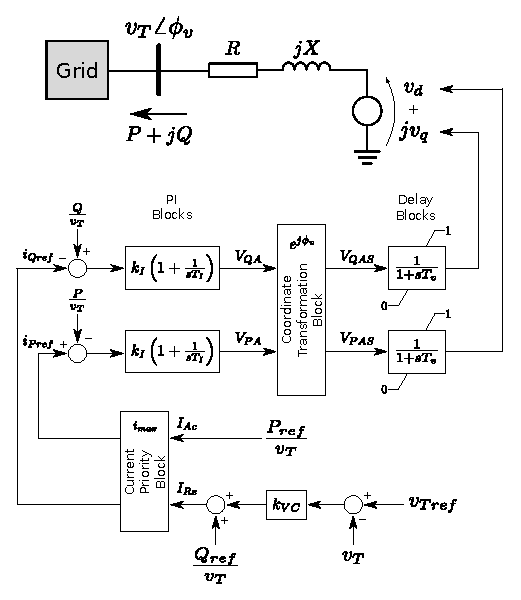
\includegraphics[scale=1]{Images/ErlichModel.eps}
	\end{center}
	\label{fig: ErlMod}
	\legend{Source: Adapted from \cite{Erlich2012}}
\end{figure}

\noindent where $v_{T}$ and $\phi_{v}$ correspond to the voltage magnitude and angle at substation bus, $P$ and $Q$ are the active and reactive power generated by the WPP, $v_{d}$ and $v_{q}$ stand for the direct and quadrature components of the generated voltage, $R$ and $X$ correspond to the Thevenin equivalent resistance and reactance, $k_{I}$ and $T_{I}$ are the PI block gain and time constant, $T_{V}$ is the delay block time constant and $k_{VC}$ is the voltage block gain.

The reference values of bus voltage ($v_{Tref}$), active ($P_{ref}$) and reactive power ($Q_{ref}$) are obtained during regime and vary according to wind speed. The real and imaginary current components that WPP must provide in order to maintain voltage and power at the reference level can be easily obtained by the equations below.

\begin{equation}
	\begin{cases}
		I_{Ac} = \frac{P_{ref}}{v_{T}} \\
		I_{Re} = k_{VC}(v_{Tref} - v_{T}) + \frac{Q_{ref}}{v_{T}}
	\end{cases}
	\label{eq: Currents}
\end{equation}

However, under certain conditions, those current components must be prioritized. Under normal conditions, the WPP must focus on delivering active power to the grid. On the other hand, in the event of voltage sag, the WPP must act on the voltage regulation, providing as much reactive power as possible. Also, under no circumstances the current limitations of the components should not be violated.

The conditions mentioned above are analysed by a current priority block. This block limits the current previously calculated by checking if it surpasses the limits allowed and if terminal voltage is below a threshold value $v^{*}$, characterizing voltage sag. Figure \ref{fig: CurrentPriority} exemplifies the block operation.

\begin{figure}
	\caption{Current priority block}
	\begin{center}
%		\includegraphics[scale=1]{Images/CurrentPriorityBlock.eps}
	\end{center}
	\label{fig: CurrentPriority}
\end{figure}

The current priority block outputs the reference values of active and reactive current that will be used to control the power generated by the WPP. The following algorithm describes the current priority block operation.

\begin{center}
	\begin{lstlisting}[mathescape, columns=fullflexible]
	if $\sqrt{I_{Ac}^{2} + I_{Re}^{2}} \leq i_{max}$ then:
		$\begin{cases}
				i_{Pref} = I_{Ac} \\
				i_{Qref} = I_{Re}
		\end{cases}$
	else:
		if $v_{T} \geq v^{*}$ then:	
			$\begin{cases}
				i_{Pref} = min(i_{max}, I_{Ac}) \\
				i_{Qref} = \sqrt{i_{max}^{2} - i_{Pref}^{2}}
			\end{cases}$
		else:
			$\begin{cases}
				i_{Qref} = min(i_{max}, I_{Re}) \\
				i_{Pref} = \sqrt{i_{max}^{2} - i_{Qref}^{2}}
			\end{cases}$
	\end{lstlisting}
\end{center}

At the next stage, proportional-integral blocks are used to represent the controllers of WTGs, specially the RSC controller. Their outputs follow the equations presented below. The values $V_{PA}$ and $V_{QA}$ are, respectively, the active and reactive voltage components (on grid coordinates) that the Thevenin voltage source must supply so the reference values of voltage and power are satisfied.

\begin{equation}
	\begin{cases}
		V_{PA} = k_{I}[(i_{Pref} - \frac{P}{v_{T}}) + \frac{1}{T_{I}}\int\displaylimits_{0}^{t} (i_{Pref} - \frac{P}{v_{T}})dt]\\
		\\
		V_{QA} = k_{I}[(\frac{Q}{v_{T}} - i_{Qref}) + \frac{1}{T_{I}}\int\displaylimits_{0}^{t} (\frac{Q}{v_{T}} - i_{Qref})dt]
	\end{cases}
	\label{eq: PI}
\end{equation}

At this point, the controllers operate on grid coordinates, so a coordinate transformation block is needed to adequate to $d-q$ coordinates. This block operates according to equation \eqref{eq: CoordShift}. It is important to notice that these equations rely on the knowledge of $\phi_{v}$ and, in order to obtain that measurement, the WPP must have a phasor measurement unit (PMU) installed on its substation.

\begin{equation}
	\begin{cases}
		V_{PAS} = -V_{PA}cos(\phi_{v}) - V_{QA}sin(\phi_{v}) \\
		V_{QAS} = V_{PA}sin(\phi_{v}) - V_{QA}cos(\phi_{v})
	\end{cases}
	\label{eq: CoordShift}
\end{equation}

Finally, limited lag blocks, simulating the delays caused by the electrical machine and converters present on WTGs, supply the voltage source. The lag block constraints limit the values of those voltage components to remain in a safety margin, between $0$ and $1$. Equation \eqref{eq: DelayBlocks} describes how these blocks affect $v_{D}$ and $v_{q}$.

\begin{equation}
	\begin{cases}
		\dot{v}_{d} = \frac{1}{T_{V}}(v_{d} - V_{PAS}) \\
		\dot{v}_{q} = \frac{1}{T_{V}}(v_{q} - V_{QAS})
	\end{cases}
	\label{eq: DelayBlocks}
\end{equation}

With direct and quadrature voltage components obtained, the power generated by the WPP can be easily calculated, as shown below.

\begin{align*}
		S^{*} &= v_{T}^{*} \cdot I = v_{T}^{*} \cdot \frac{[(v_{d} + jv_{q}) - v_{T}]}{R + jX} \\
		\\
		&= (v_{Td} - jv_{Tq})\cdot\left[\frac{v_{d} + jv_{q} - (v_{Td} + jv_{Tq})}{R + jX}\right]\cdot \frac{R - jX}{R - jX} \\
		\\
		&= \frac{v_{Td}v_{d} + v_{Tq}v_{q} - v_{T}^{2} + j(v_{Td}v_{q} - v_{Tq}v_{d})}{R^{2} + X^{2}}\cdot (R - jX) \\
		\\
		&= \frac{R(v_{Td}v_{d} + v_{Tq}v_{q} - v_{T}^{2}) + X(v_{Td}v_{q} - v_{Tq}v_{d})}{R^{2} + X^{2}} - j\frac{X(v_{Td}v_{d} + v_{Tq}v_{q} - v_{T}^{2}) - R(v_{Td}v_{q} - v_{Tq}v_{d})}{R^{2} + X^{2}} \\
\end{align*}

Thus,

\begin{equation}
	\begin{cases}
		P = \frac{R(v_{Td}v_{d} + v_{Tq}v_{q} - v_{T}^{2}) + X(v_{Td}v_{q} - v_{Tq}v_{d})}{R^{2} + X^{2}} \\
		Q = \frac{X(v_{Td}v_{d} + v_{Tq}v_{q} - v_{T}^{2}) - R(v_{Td}v_{q} - v_{Tq}v_{d})}{R^{2} + X^{2}}
	\end{cases}
	\label{eq: Outputs}
\end{equation}

The summarized model is shown below.

\begin{equation}
	\begin{cases}
		\dot{v}_{d} = \frac{1}{T_{V}}(v_{d} - V_{PAS}) \\
		\dot{v}_{q} = \frac{1}{T_{V}}(v_{q} - V_{QAS}) \\
		\\
		P = \frac{R(v_{Td}v_{d} + v_{Tq}v_{q} - v_{T}^{2}) + X(v_{Td}v_{q} - v_{Tq}v_{d})}{R^{2} + X^{2}} \\
		Q = \frac{X(v_{Td}v_{d} + v_{Tq}v_{q} - v_{T}^{2}) - R(v_{Td}v_{q} - v_{Tq}v_{d})}{R^{2} + X^{2}} \\
		\\
		V_{PAS} = -V_{PA}cos(\phi_{v}) - V_{QA}sin(\phi_{v}) \\
		V_{QAS} = V_{PA}sin(\phi_{v}) - V_{QA}cos(\phi_{v}) \\
		\\
		V_{PA} = k_{I}[(i_{Pref} - \frac{P}{v_{T}}) + \frac{1}{T_{I}}\int\displaylimits_{0}^{t} (i_{Pref} - \frac{P}{v_{T}})dt]\\
		V_{QA} = k_{I}[(\frac{Q}{v_{T}} - i_{Qref}) + \frac{1}{T_{I}}\int\displaylimits_{0}^{t} (\frac{Q}{v_{T}} - i_{Qref})dt]
	\end{cases}
	\label{eq: Summary}
\end{equation}

\begin{center}
	\begin{lstlisting}[mathescape, columns=fullflexible]
	if $\sqrt{I_{Ac}^{2} + I_{Re}^{2}} \leq i_{max}$ then:
		$\begin{cases}
				i_{Pref} = I_{Ac} \\
				i_{Qref} = I_{Re}
		\end{cases}$
	else:
		if $v_{T} \geq v^{*}$ then:	
			$\begin{cases}
				i_{Pref} = min(i_{max}, I_{Ac}) \\
				i_{Qref} = \sqrt{i_{max}^{2} - i_{Pref}^{2}}
			\end{cases}$
		else:
			$\begin{cases}
				i_{Qref} = min(i_{max}, I_{Re}) \\
				i_{Pref} = \sqrt{i_{max}^{2} - i_{Qref}^{2}}
			\end{cases}$
	\end{lstlisting}
\end{center}

\begin{equation*}
	\begin{cases}
		I_{Ac} = \frac{P_{ref}}{v_{T}} \\
		I_{Re} = k_{VC}(v_{Tref} - v_{T}) + \frac{Q_{ref}}{v_{T}}
	\end{cases}
\end{equation*}

Thus, this model can be interpreted as presented in \eqref{eq: xdot}, where the state variable ($x$), input ($u$), output ($y$) and parameter ($p$) vectors are described by \eqref{eq: x}, \eqref{eq: u}, \eqref{eq: y} and \eqref{eq: p}, respectively.

\begin{equation}
	\begin{cases}
		\dot{x} = f(x, y, p, u) \\
		y = g(x, p, u)
	\end{cases}
	\label{eq: xdot}
\end{equation}

\begin{equation}
	x = [v_{d}, v_{q}]^T
	\label{eq: x}
\end{equation}

\begin{equation}
	u = [v_{T}, \phi_{v}, P, Q]^T
	\label{eq: u}
\end{equation}

\begin{equation}
	y = [P, Q]^T
	\label{eq: y}
\end{equation}

\begin{equation}
	p = [R, X, k_{I}, T_{I}, T_{V}, k_{VC}, i_{max}]^T
	\label{eq: p}
\end{equation}

The parameters presented in \eqref{eq: p} are the subject of the estimation process presented on the next chapter. Those values define the behaviour of wind power plants during disturbances.

\subsection{Proposed Model for Further Studies}

One of the disadvantages of the model presented above is the need of information about voltage angle $\phi_{v}$. In order to acquire angle measurements, the grid must have special equipments, such as PMUs, installed on some of its buses. However, by dislocating the coordinate transformer block to a point before the WPP bus, $\phi_{v}$ may be excluded from the model. Figure \ref{fig: Proposed_Model} depicts the block diagram of the proposed model.

\begin{figure}[h]
	\caption{WPP model proposed by author}
	\begin{center}
		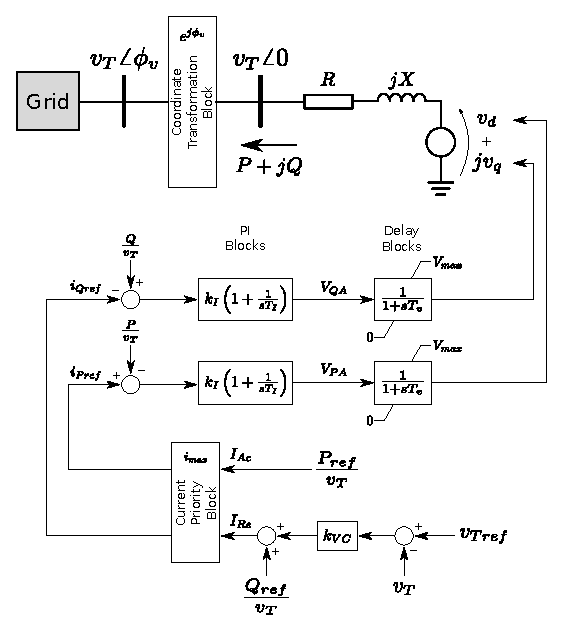
\includegraphics[scale=1]{Images/proposed_model.eps}
	\end{center}
	\label{fig: Proposed_Model}
\end{figure}

The equations of this model are slightly altered by this change, with \eqref{eq: DelayBlocks} and \eqref{eq: Outputs} becoming \eqref{eq: DelayBlocks_new} and \eqref{eq: Outputs_new}, respectively. Also, the limits applied to the delay blocks also change and must be further investigated.

\begin{equation}
	\begin{cases}
		\dot{v}_{d} = \frac{1}{T_{V}}(v_{d} - V_{PA}) \\
		\dot{v}_{q} = \frac{1}{T_{V}}(v_{q} - V_{QA})
	\end{cases}
	\label{eq: DelayBlocks_new}
\end{equation}

\begin{equation}
	\begin{cases}
		P = \frac{R(v_{T}v_{d} - v_{T}^{2}) - Xv_{T}v_{q}}{R^{2} + X^{2}} \\
		Q = \frac{X(v_{T}v_{d} - v_{T}^{2}) - Rv_{T}v_{q}}{R^{2} + X^{2}}
	\end{cases}
	\label{eq: Outputs_new}
\end{equation}

The vectors $x$, $y$ and $p$ remain the same on this new model and the new input vector $u$ is given by:

\begin{equation}
	u = [v_{T}, P, Q]^T
	\label{eq: u_new}
\end{equation}
% ---
% Capítulo 3 - Parameter Estimation Process
% ---
\chapter{Parameter Estimation Process}

\label{ch: Estim}

Parameter estimation problems can be interpreted as optimization problems, where one must find the optimal values of parameters in order to reduce the error between real system and model outputs when the same disturbance is applied to it. The error $J(p)$ is evaluated using the L2-norm, given by equation \eqref{eq: J(p)}, where $y_{r}$ and $y$ stand for the real system and model outputs, respectively. During years, many methods were developed to address this problem, but two approaches have been largely employed to obtain its solution.

\begin{equation}
	J(p) = \frac{1}{2}\int\displaylimits_{0}^{T_{0}}(y_{r}(t) - y(t))^{T}(y_{r}(t) - y(t))dt
	\label{eq: J(p)}
\end{equation}

The first approach applies metaheuristics to obtain a sufficiently good solution. These methods are used in a variety of cases, ranging from biological to engineering problems, due to the fact that they are not developed for a specific type of problem. Metaheuristics employ a stochastic search to find (near-)optimal solutions inside a given region. However, those methods often take a great amount of time to converge to a solution \cite{Blum2003}. Examples of metaheuristics are Ant Colony Optimization, Differential Evolution, Particle Swarm Optimization and Genetic Algorithm. Applications of this approach in electrical power system cases can be found in \cite{Todorovski2006} and \cite{Yoshida2000}.

The second approach applies analytical methods to find the local optimum solution from equations derived from the problem. Thus, they are problem specific and must be adapted from one case to another. Analytical methods often converge in few iterations, reducing processing time, but they are sensitive to initial conditions. Some examples of analytical methods are Newton's Method, Kalman Filter, Unscented Kalman Filter, etc.

By combining both approaches, is expected to reduce the effects of their disadvantages and improving overall convergence. Mean-Variance Mapping Optimization (MVMO) was the metaheuristic chosen for this problem, alongside Trajectory Sensitivity Method (TSM) as analytical method. Both methods will be discussed in the following sections.

\section{Mean-Variance Mapping Optimization Method}

Presented in \cite{Erlich2010}, this metaheuristic based in evolution of populations shares characteristics with other evolutionary algorithms, but differ from them on how to induce mutations on the offspring in order to diversify the population. By considering statistical data of population during mutation process, MVMO introduces a memory factor to it, enhancing search mechanism. Due this factor, MVMO performs better than similar metaheuristics when population size is relatively small \cite{Nakawiro2011}. The terms `gene', `individuals' and `population' refer to `parameter', `parameter vector' and `set of parameter vectors' in MVMO, for the sake of analogy.

Two other relevant concepts largely used on metaheuristics are exploration and exploitation. The first one refers to a broad search carried through the region of interest. On the other hand, exploitation means the search on a small neighbourhood close to the best solutions.

Before starting the parameter search process, a few settings must be done, such as population size, number of offspring, number of genes selected for mutation and selection method. Also, the search region is defined by setting the range within genes can vary. This constrains the parameters values within a feasible region, preventing divergence. The search region is later normalized for all genes, aiding the estimation process. Termination criteria is also set in this step. In this work, both number of generations and error will be used as stop criteria.

After that, a randomly-distributed population is generated, evaluated and sorted. Moreover, the mean and variance of every gene in each population are calculated. These values will later be used on the mutation process. The individual with lower error is selected as parent for a new generated individual. The offspring is then created following three steps common in evolutionary algorithms: gene selection, mutation and crossover. After creation, the offspring is introduced to the population and the worst individual is discarded, as depicted in Figure \ref{fig: MVMOprocess}.

\begin{figure}[h]
	\caption{Exemplification of MVMO process}
	\begin{center}
		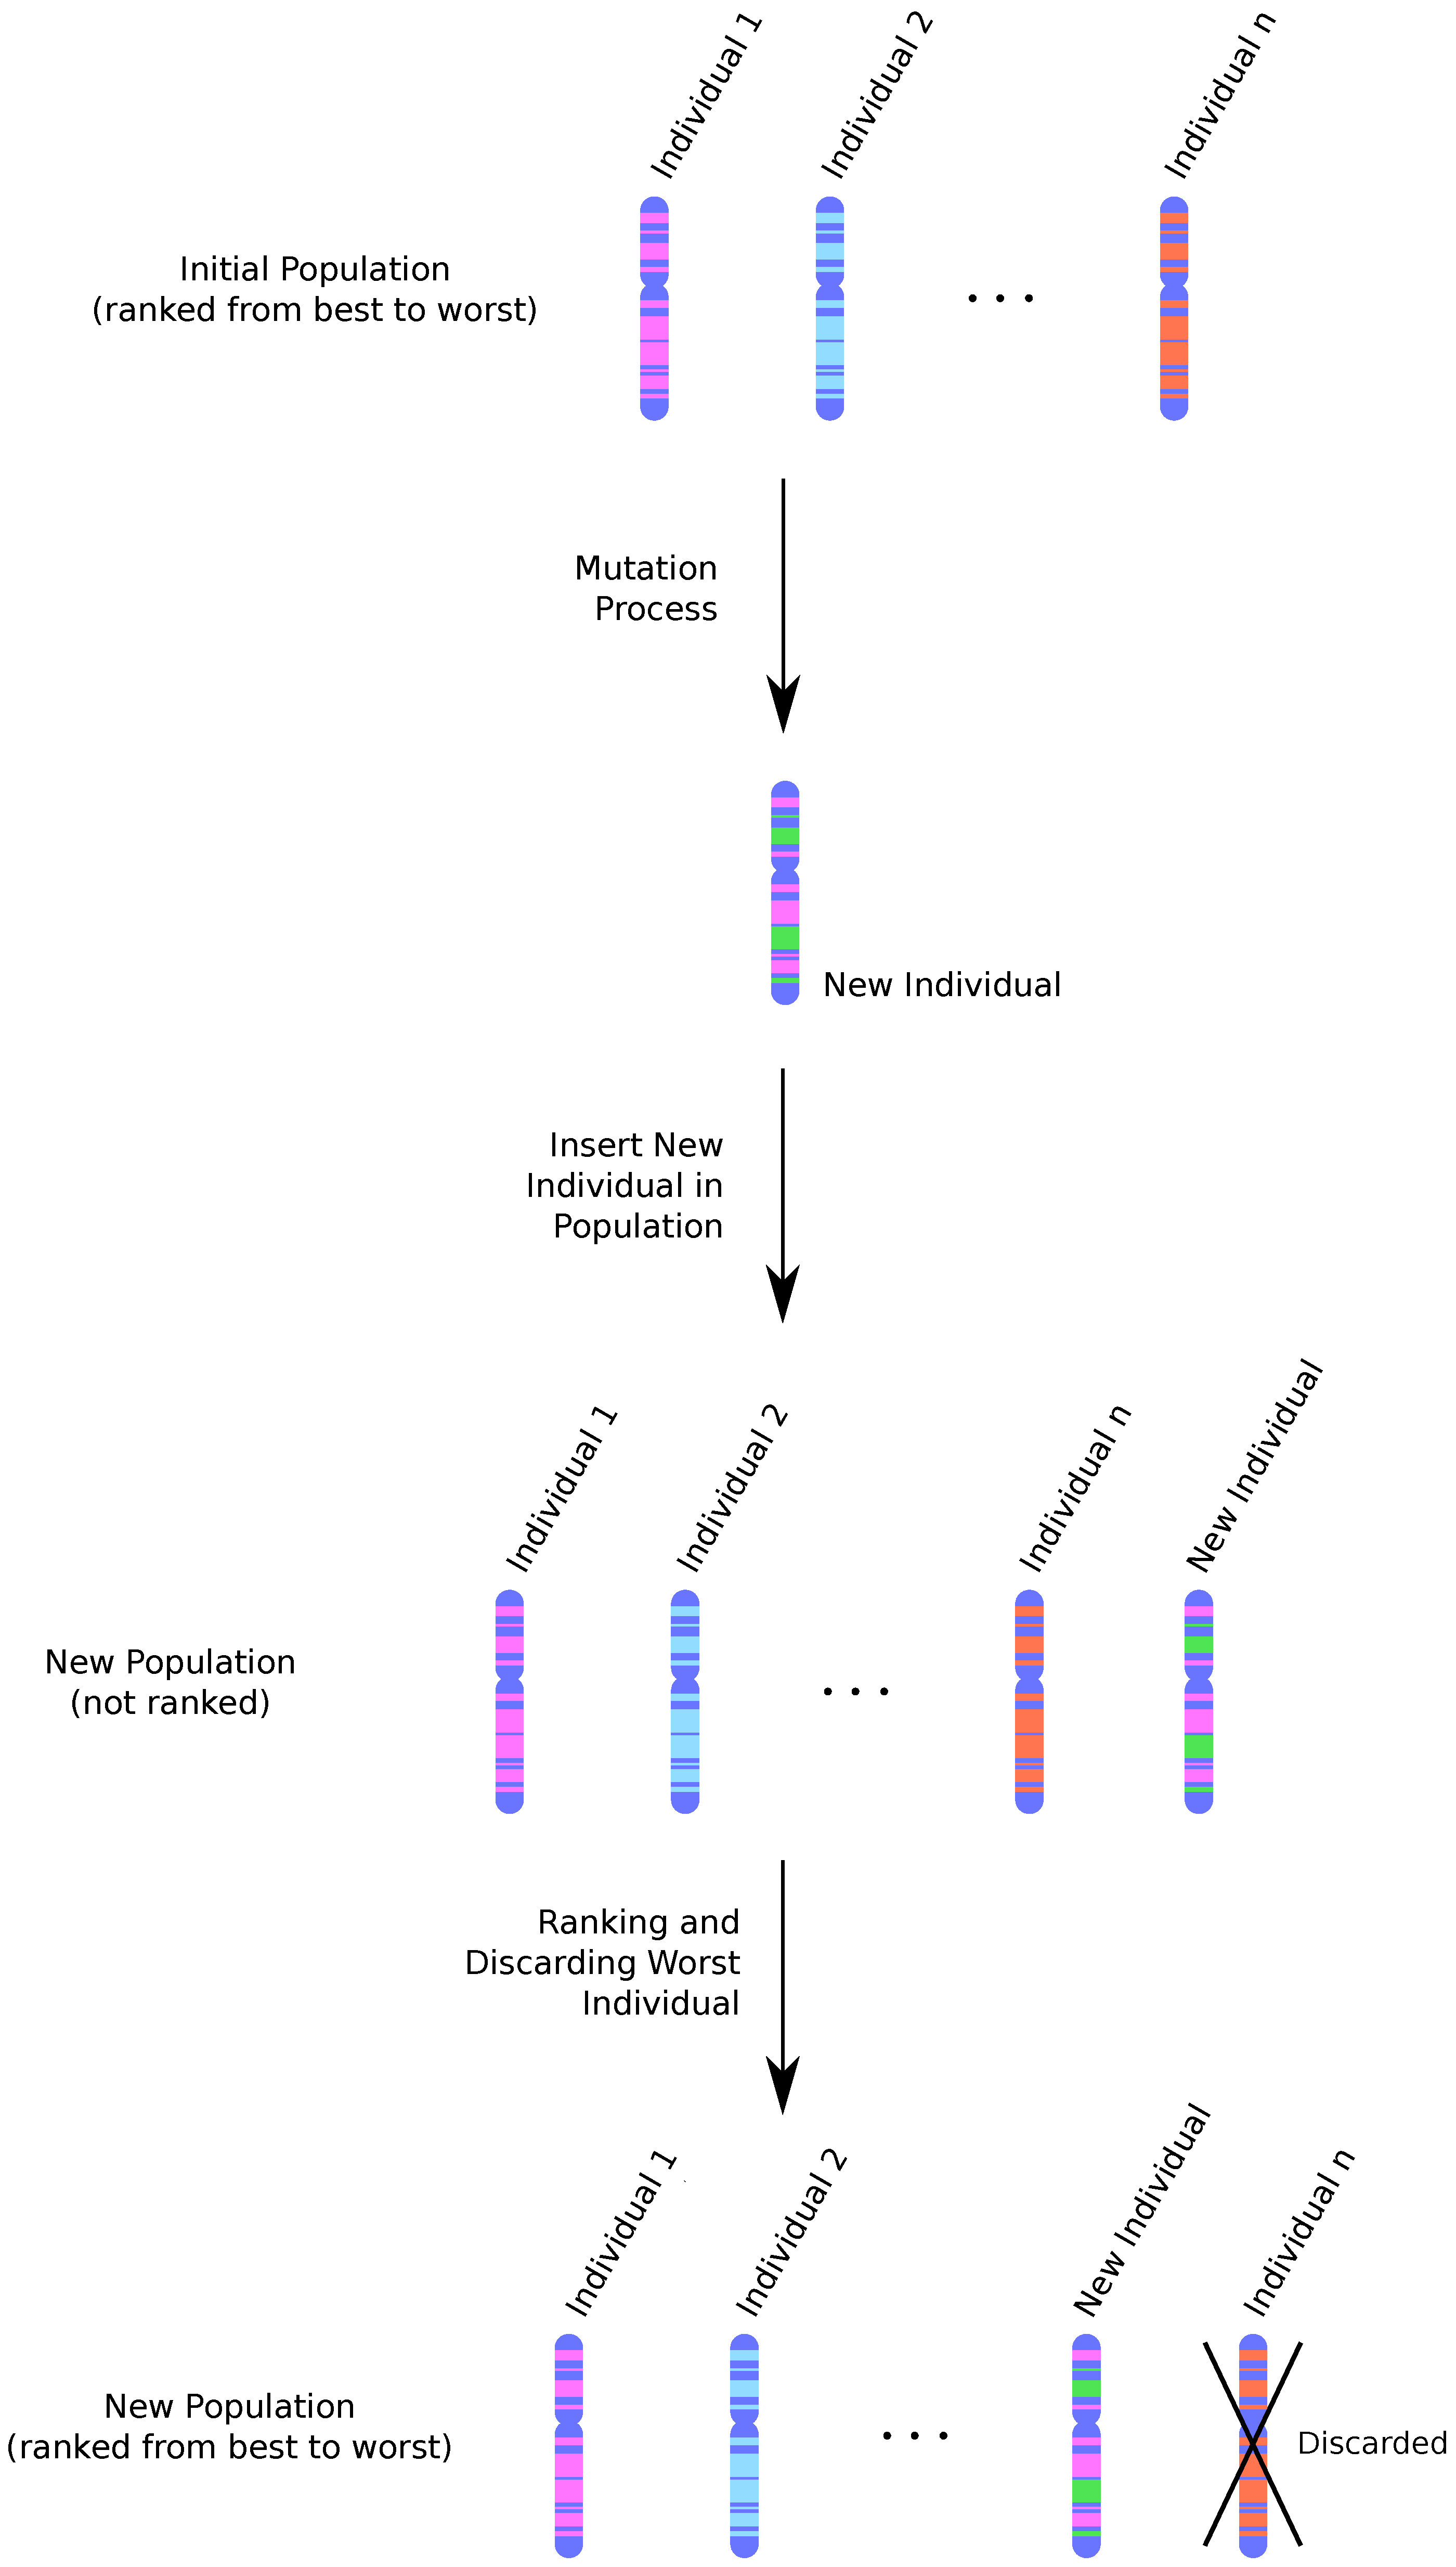
\includegraphics[scale=.2]{Images/MVMO_process2.eps}
	\end{center}
	\label{fig: MVMOprocess}
\end{figure}

\textbf{Gene selection} can be done in many ways and even vary throughout the estimation process, with strategies' efficiency depending on the problem. However, three strategies are commonly used in this step. The first one is comprised of randomly selecting which genes will suffer mutation and which will be directly inherited from the parent. Gene selection can also be done by a moving window approach or even a combination of both strategies, with part of the genes selected at random and other through the window.

\textbf{Mutation} step takes place after gene selection. At first, each selected gene receives a random value $\tilde{p}$ between [0,1] that will be used as an input to a mapping function based on the mean and variance of each particular gene on the population. Variance $v_{i}$ will directly influence on the shape factor $s_{i}$,  given by \eqref{eq: shapefac}, where $f_{s}$ is the scaling factor responsible for focusing on exploration or exploitation. In the event of zero variance, the last non-null value of $v_{i}$ is used.

\begin{equation}
	s_{i} = -f_{s}ln(v_{i})
	\label{eq: shapefac}
\end{equation}

Shape factor and mean value of genes of the population are used as inputs to a transformation function $h$, detailed in \eqref{eq: hfunc}. The final value of the gene is obtained through the mapping function described by equation \eqref{eq: mappingf}, where $h_{p} = h(u_{i} = \tilde{p})$, $h_{1} = h(u_{i} = 1)$ and $h_{0} = h(u_{i} = 0)$. It is important to notice that the mapping function will always provide a result in the interval [0,1], not violating the normalization made at beginning.

\begin{equation}
	h(\bar{p_{i}}, s_{i1}, s_{i2}, u_{i}) = \bar{p_{i}}(1 - e^{-u_{i}s_{i1}}) + (1 + \bar{p_{i}})e^{-(1 - u_{i})s_{i2}}
	\label{eq: hfunc}
\end{equation}

\begin{equation}
	p_{i} = h_{p} + (1 - h_{1} + h_{0})\tilde{p} - h_{0}
	\label{eq: mappingf}
\end{equation}

The resulting mapping function is depicted in Figure \ref{fig: mappingf}. The effects of different mean and shape factor values can be observed on Figure \ref{fig: mapeffects}.

\begin{figure}[!h]
	\caption{Example of MVMO mapping function}
	\begin{center}
		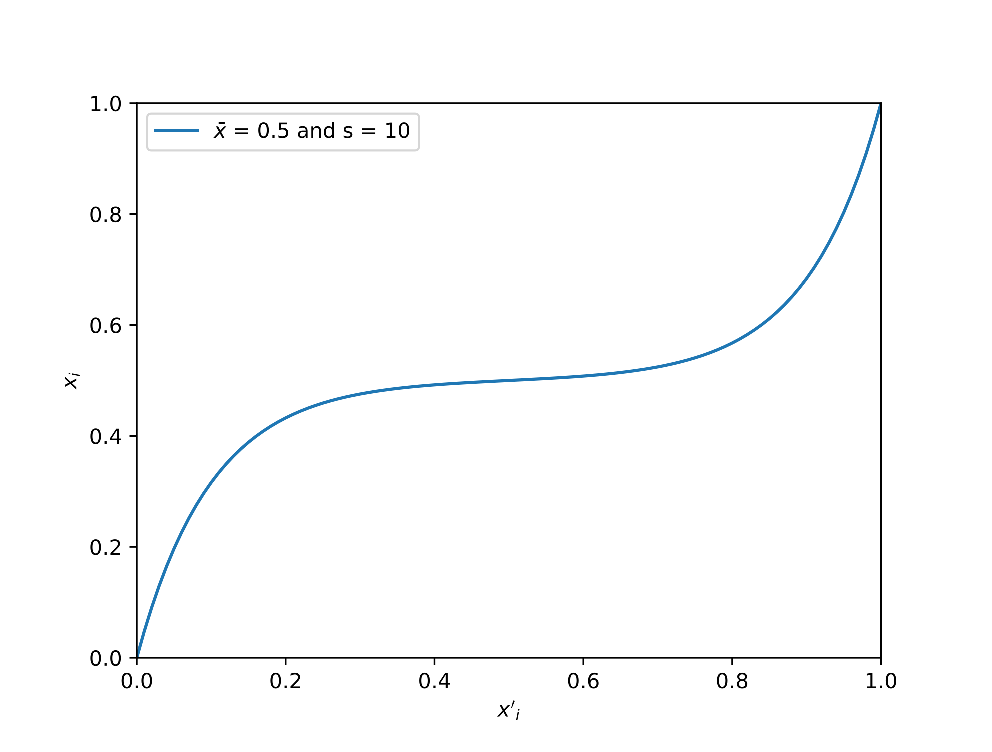
\includegraphics[scale=.5]{Images/MVMOTransformation.eps}
	\end{center}
	\label{fig: mappingf}
\end{figure}

\begin{figure}[h]
	\caption{Effect of different mean and shape factor values on mapping function}
	\begin{center}
		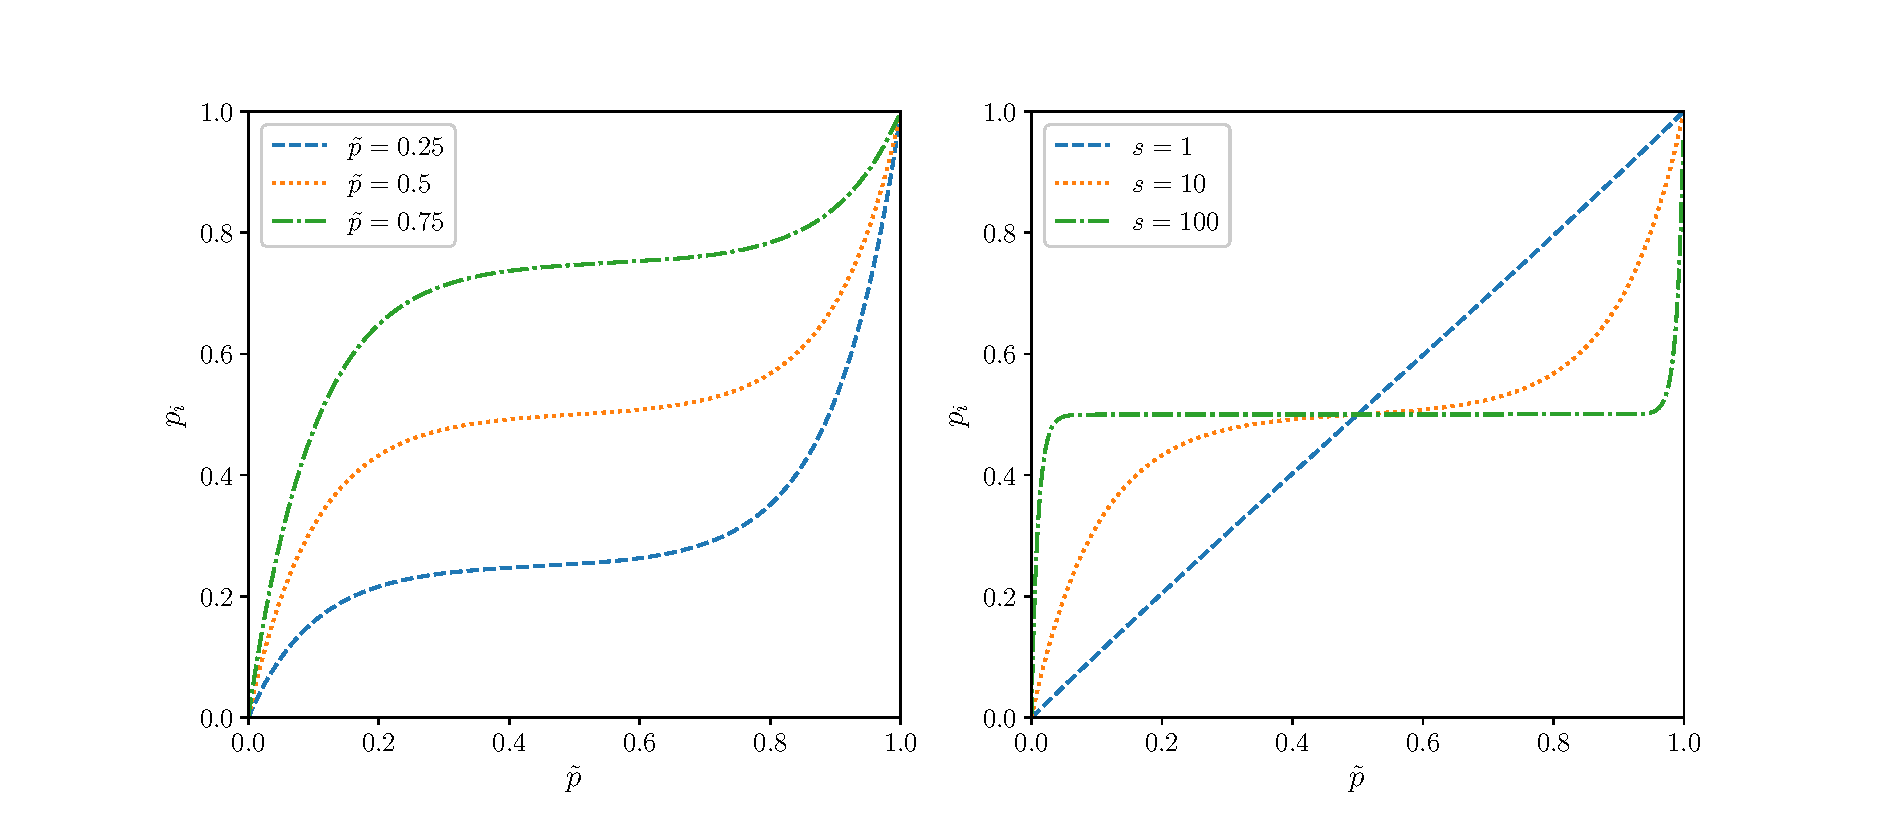
\includegraphics[scale=.5]{Images/mean_var_effects.eps}
	\end{center}
	\label{fig: mapeffects}
\end{figure}

As shown in \eqref{eq: hfunc}, two shape factors are used to evaluate the function. Different values of shape factors emphasizes the search below or above mean value. Thus, by controlling the values $s_{i1}$ and $s_{i2}$, the method can prioritize exploration (global search) or exploitation (local search) on a given region. Figure \ref{fig: diffs} depicts how asymmetrical shape factors affect the mapping function.

\begin{figure}[h]
	\caption{Comparison between symmetrical and asymmetrical shape factors}
	\begin{center}
		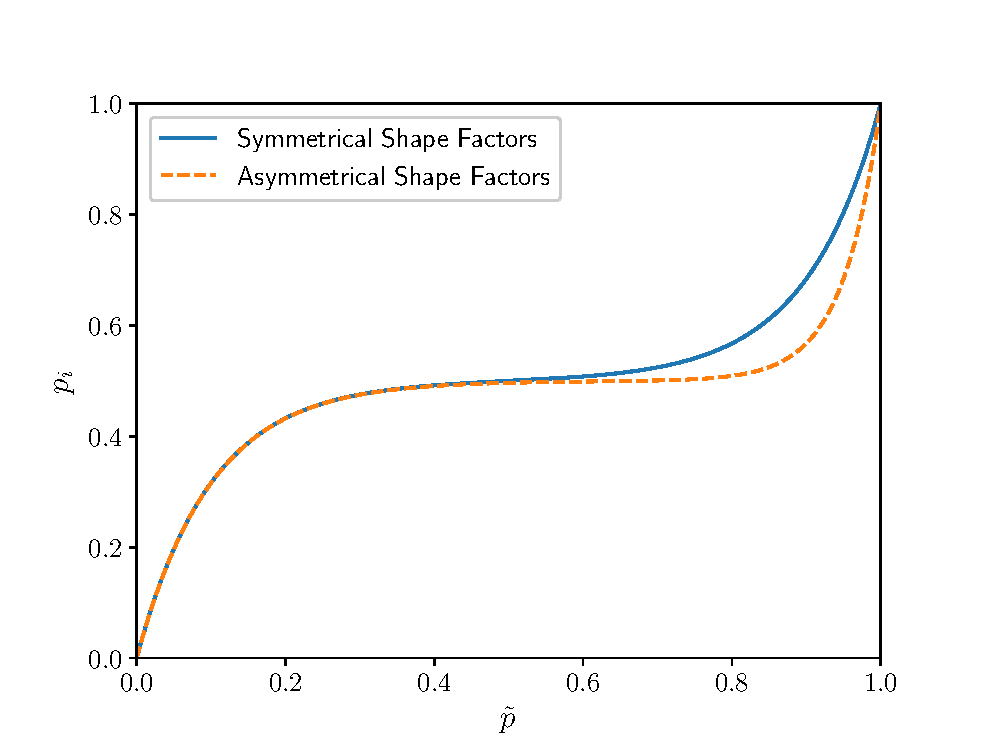
\includegraphics[scale=.5]{Images/symmetrical_transf.eps}
	\end{center}
	\label{fig: diffs}
\end{figure}

The final step during offspring generation is crossover. During this phase, the mutated genes are united with the remaining genes inherited from parent, forming the new individual. This new individual is evaluated and included to the population if it is better than, at least, the population's worst individual. This process goes on until at least one stop criterion has been fulfilled.

The main advantages of this method are low computational cost, good performance using small populations, constrained search region, preventing divergence, and the fact that it is non-specific. On the other hand, this method, as other metaheuristics, takes a great amount of time to converge when its error approaches zero.

\section{Trajectory Sensitivity Method}

Considering a nonlinear system described by \eqref{eq: xdot}, in order to minimize the error between model and real system, given by \eqref{eq: J(p)}, one must discover a parameter vector $p^{*}$ such as:

\begin{equation}
	G(p^{*}) = \frac{\partial J(p^{*})}{\partial p} = 0
\end{equation}

This derivative can be written as:

\begin{equation}	
	G(p) = -\int\displaylimits_{0}^{T_{0}} \left(\frac{dy}{dp}\right)^{T} (y_{r} - y) dt
	\label{eq: G(p)}
\end{equation}

Truncating the Taylor series for $G(p)$ on the first-order term results on \eqref{eq: Taylor}. The matrix $\Gamma$ is described in \eqref{eq: Gamma}.

\begin{equation}
	G(p^{*}) = G(p) + \Gamma (p)(p^{*} - p)
	\label{eq: Taylor}
\end{equation}

\begin{equation}
	\Gamma (p) = \frac{\partial G(p)}{\partial p} \approx \int\displaylimits_{0}^{T_{0}} \left(\frac{dy}{dp}\right)^{T} \left(\frac{dy}{dp}\right) dt
	\label{eq: Gamma}
\end{equation}

By rearranging the terms on \eqref{eq: Taylor}, the following equation is obtained. It describes how the parameters are updated after the $n^{th}$ iteration.

\begin{equation}
	p^{n+1} = p^{n} + \Gamma^{-1}(p^{n})\cdot G(p^{n})
\end{equation}

Obtaining the Jacobian matrix (also called trajectory sensitivity matrix) $\frac{\partial y}{\partial p}$, used in \eqref{eq: G(p)} and \eqref{eq: Gamma}, analytically is a hard task. However, by applying the definition of derivative, given by \eqref{eq: deriv}, the sensibilities can be approximated without any analytical derivation of the equations.

\begin{equation}
	\frac{df(x)}{dx} = \lim\limits_{\delta \to 0} \frac{f(x + \delta) - f(x)}{\delta}
	\label{eq: deriv}
\end{equation}

Consider two parameter vectors $p$ and $p^{\epsilon}$, where $p^{\epsilon}$ is obtained by adding a small perturbation $\epsilon p_{i}$ to the $i-th$ element of $p$, as shown in \eqref{eq: pvecs}.

\begin{equation}
	p = 
	\begin{bmatrix}
		p_{1} \\
		\vdots \\
		p_{i} \\
		\vdots \\
		p_{n}
	\end{bmatrix}; \ \ \ \ 
	 p^{\epsilon} =
	\begin{bmatrix}
		p_{1} \\
		\vdots \\
		p_{i} + \epsilon p_{i} \\
		\vdots \\
		p_{n}
	\end{bmatrix}
	\label{eq: pvecs}
\end{equation}

With $\epsilon$ sufficiently small, the partial derivative with respect to the parameter $p_{i}$ can be approximated by the difference shown in equation \eqref{eq: diff}. The value of $\epsilon = 0.1 \times 10^{-3}$ have shown great results for most cases. Using the approximation of the partial derivatives allows Trajectory Sensitivity method to be applied on both differentiable and non-differentiable systems \cite{Benchluch1993}, \cite{Cari2006}.

\begin{equation}
	\frac{\partial y(x, p, u)}{\partial p_{i}} \approx \frac{y(x, p^{\epsilon}, u) - y(x, p, u)}{\epsilon p_{i}}
	\label{eq: diff}
\end{equation}

The Trajectory Sensitivity Method has fast convergence characteristics and can applied directly to nonlinear problems, not requiring linearization. Also, by analyzing the sensitivities, the method provides information about identifiability of parameters. However, TSM is very sensitive to initial value of parameter chosen as starting point. Thus, if the initial values are too far from the real values, the method can either diverge or converge to wrong values. Besides, the information provided to the method must contain the effects of the parameters, otherwise they won't be observable \cite{Benchluch1993}.

\section{Hybrid Estimation Method}

By associating MVMO and TSM, the hybrid estimation approach applied in this work combines most benefits of both methods whilst mitigating their disadvantages. The resulting method has smaller convergence time when compared to MVMO alone and is less sensitive to initial values of parameters than TSM.

The flowchart depicted in Figure \ref{fig: flowchart} illustrates how this method works. At first, a disturbance occurs, resulting in a dynamic response of the real system. While $J(p)$ is greater than a given tolerance $tol_{1}$, MVMO algorithm will look for possible optimal solutions across the search region. Afterwards, the error will eventually drop to a value lower than $tol_{1}$, and TSM will be used to refine the search to an optimal solution, with error level below tolerance $tol_{2}$.

\begin{figure}[!h]
	\caption{Flowchart of estimation method}
	\begin{center}
		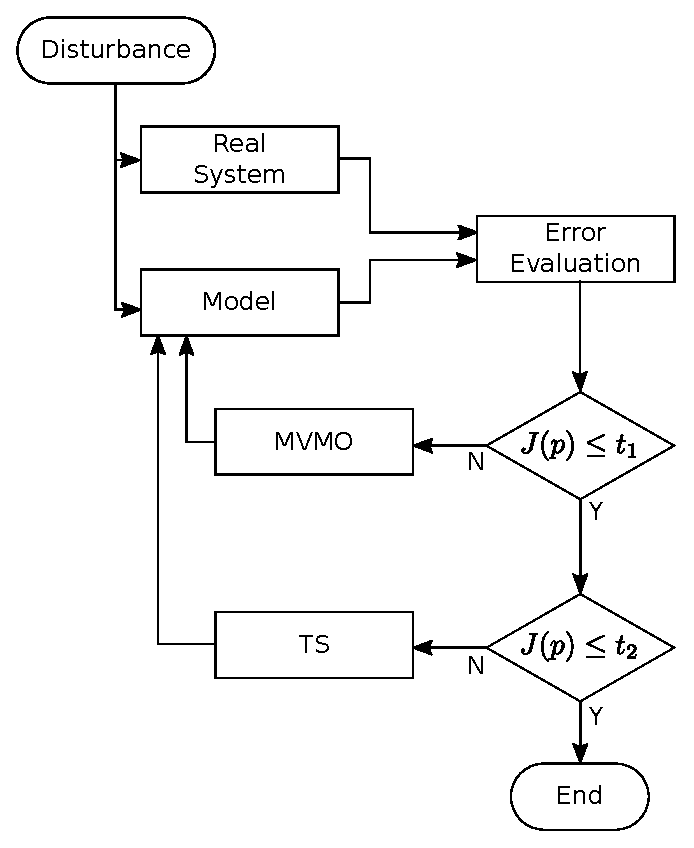
\includegraphics[scale=0.7]{Images/Flowchart.eps}
	\end{center}
	\label{fig: flowchart}
\end{figure}

% ---
% Capítulo 4 - Software
% ---
\chapter{Software Concept}

\label{ch: software}

In this chapter, the concept behind the software in development is presented. The entire software will be developed using Python, a powerful, simple and fast high-level programming language that has gained large space in various sectors of industry and academy. Its rise is due mainly to the enormous number of libraries and forums developed and maintained by the users. Some examples of libraries used in this project are numpy (for scientific computing), matplotlib (plotting library), Tkinter and Qt (Graphical User Interface toolkit). Python is also open-source, not requiring a paid software to code and most of its applications are free.

Although the estimation method and mathematical model that are subject of this work, the software in development will not be specific to them. Instead, it will be generic and both model and method may be imported as packages. This will allow future users to employ it on different applications concerning parameter estimation. Also, comparison between method's performance and model's precision can be easily done with this software.

In order to improve the experience of users, a Graphical User Interface (GUI) will be developed. It will provide an simple environment for all users, so they won't need to go through the code to change any settings. Instead, the settings will be done at the beginning of the process and follow a predefined order.

The start page will display some information about the software and the parameter estimation process. Next, the user will choose from a list which mathematical model will be employed. After that, a list of identification methods will be presented and the user will be able to pick up to two methods. The settings of the chosen methods will done on the following windows and, finally, the user will enter the file containing the real system data and point out which data will be used as input and output. With all set, the estimation process will start and at its end a report will display the estimated parameters and the comparison between real system and model behaviours. 

The order presented is not definitive and may change throughout the project if needed. However, all the steps discussed are core to the estimation process and cannot be discarded. Also, some other steps may be included in order to improve the software.
% ---
% Capítulo 5 - Results
% ---
\chapter{Results}
\label{ch: Results}

The estimation package was applied on the mathematical model presented in Section \ref{sec: WPP_model}, developed to represent wind power plants. The hybrid estimation method presented in Section \ref{sec: Hybrid_Method} was applied, with MVMO providing a smart initial solution that will be refined by TSM. The results of the estimation process are shown in the following section of this chapter. A study on the effects of population size on MVMO convergence time was also made and its results are depicted below. Simulations using the proposed model are also presented in this chapter.

Besides, in order to evaluate the package support on models of different systems, it was used to estimate the parameters of a Spring-Mass system and a Linearized Z-IM Load Model. The estimation of these models is presented in the appendices.

\section{Estimation of Original WPP Model}

The estimation was conducted using the disturbance data collected in \cite{Cari2015} as the real system output. In said study, a fault was simulated on a test system using \textit{PowerFactory 14} and the data was used to estimate the parameters of the WPP model using only TSM. The system was simulated during $1\ s$ with measurements taken every $0.001\ s$. The fault was applied at $t=0.1\ s$ and was cleared out by the protection devices at $t=0.3\ s$. Figure \ref{fig: test_system} displays the test system used to collect data and Figure \ref{fig: WPP_voltage} depicts the WPP bus voltage measured during simulation.

\begin{figure}[!h]
	\caption{Test system simulated}
	\begin{center}
		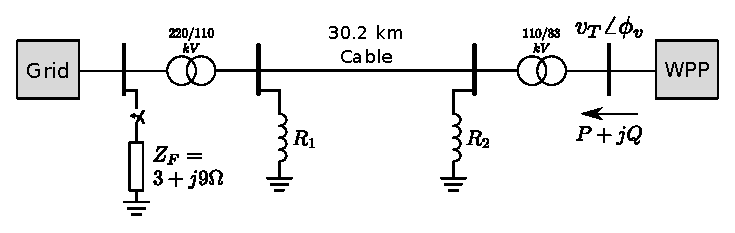
\includegraphics[scale=1]{Images/Cari_test_system.eps}
	\end{center}
	\label{fig: test_system}
\end{figure}

\begin{figure}[!h]
	\centering
	\caption{WPP bus voltage}
	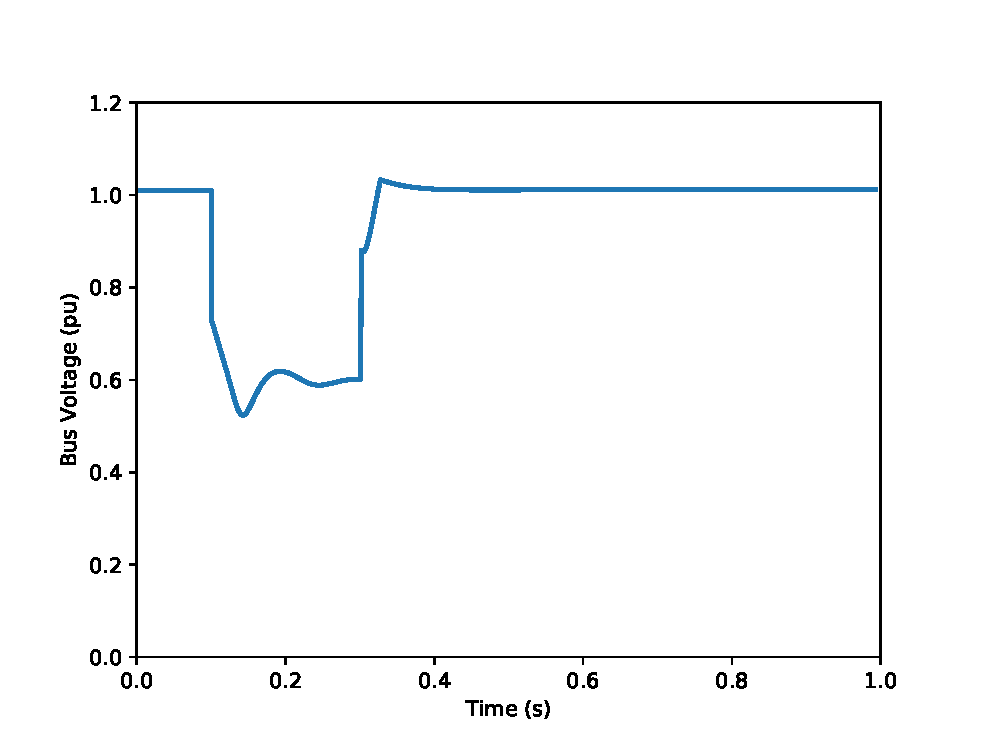
\includegraphics[scale=.7]{Images/bus_voltage.eps}
	\label{fig: WPP_voltage}
\end{figure}

MVMO search region was defined as depicted in Table \ref{tab: MVMO_boundaries}. These boundaries were decided based on the values previously found in \cite{Cari2015}.

\begin{table}[!h]
	\centering
	\caption{MVMO search region}
	\begin{tabular}{c|cc}
		Parameter & \shortstack{Lower \\ boundary} & \shortstack{Upper \\ boundary} \\\hline
		R & 0.027 & 0.040 \\
		X & 0.16 & 0.24 \\
		$k_{I}$ & 5.58 & 8.37 \\
		$T_{I}$ & 0.028 & 0.043 \\
		$T_{V}$ & 0.22 & 0.32 \\
		$k_{VC}$ & 1.60 & 2.40 \\
		$i_{max}$ & 0.88 & 1.32
	\end{tabular}
	\label{tab: MVMO_boundaries}
\end{table}

At first, 15 individuals (set of parameters) were randomly generated inside this given region, evaluated and ranked according to their error $J$. At every generation, three parameters of the fittest individual would suffer mutation in order to generate a new individual. This process continued until the fittest individual reached an error level below a tolerance of $tol_{1} = 0.5$. If this criterion were not met, MVMO would halt when the \nth{5000} generation was reached.

The fittest individual found by MVMO was then used as the starting point to TSM. Since this method converges quickly when close to the optimal solution, it was configured to run for only 7 iterations. Its goal was to find a set of parameters with $J(p)$ below $tol_{2} = 5\times10^{-4}$.

The parameters were estimated in 8.11 seconds in total, with MVMO and TSM taking 4.19 and 3.92 seconds, respectively, resulting in an error $J(p)$ of $1.5\times 10^{-4}$. The value estimated for each parameter is displayed in the Table \ref{tab: results}.

\begin{table}[h]
	\centering
	\caption{Estimated values of parameters}
	\begin{tabular}{c|c}
		Parameter & \shortstack{Estimated \\ value} \\\hline
		R & 0.034 \\
		X & 0.198 \\
		$k_{I}$ & 6.333 \\
		$T_{I}$ & 0.0348 \\
		$T_{V}$ & 0.246 \\
		$k_{VC}$ & 1.999 \\
		$i_{max}$ & 1.100
	\end{tabular}
	\label{tab: results}
\end{table}

Figures \ref{fig: output_P} and \ref{fig: output_Q} depict, respectively, real and active power measured from the simulated system and calculated using the WPP model with estimated parameters. For both components, the model output matches almost exactly with the curve expected. Therefore, the WPP model adjusted with the parameter vector found is able to reproduce the behaviour of the same wind power plant in similar conditions.

\begin{figure}[h]
	\centering
	\caption{Active power measured and modelled.}
	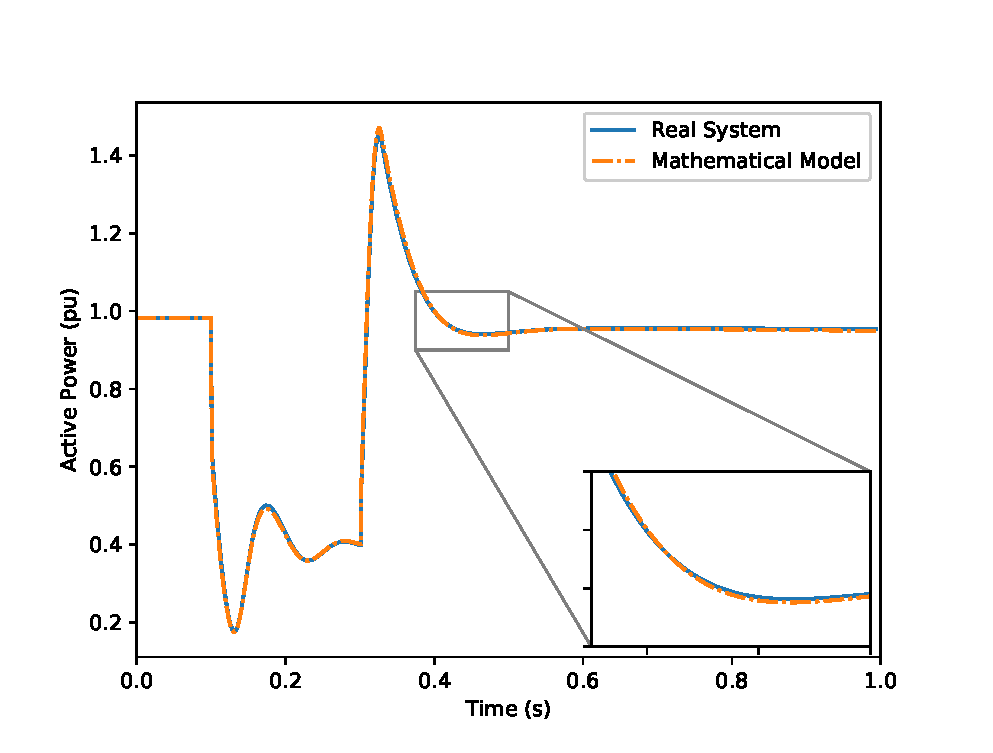
\includegraphics[scale=0.7]{Images/P_compared.eps}
	\label{fig: output_P}
\end{figure}

\begin{figure}[h]
	\centering
	\caption{Reactive power measured and modelled.}
	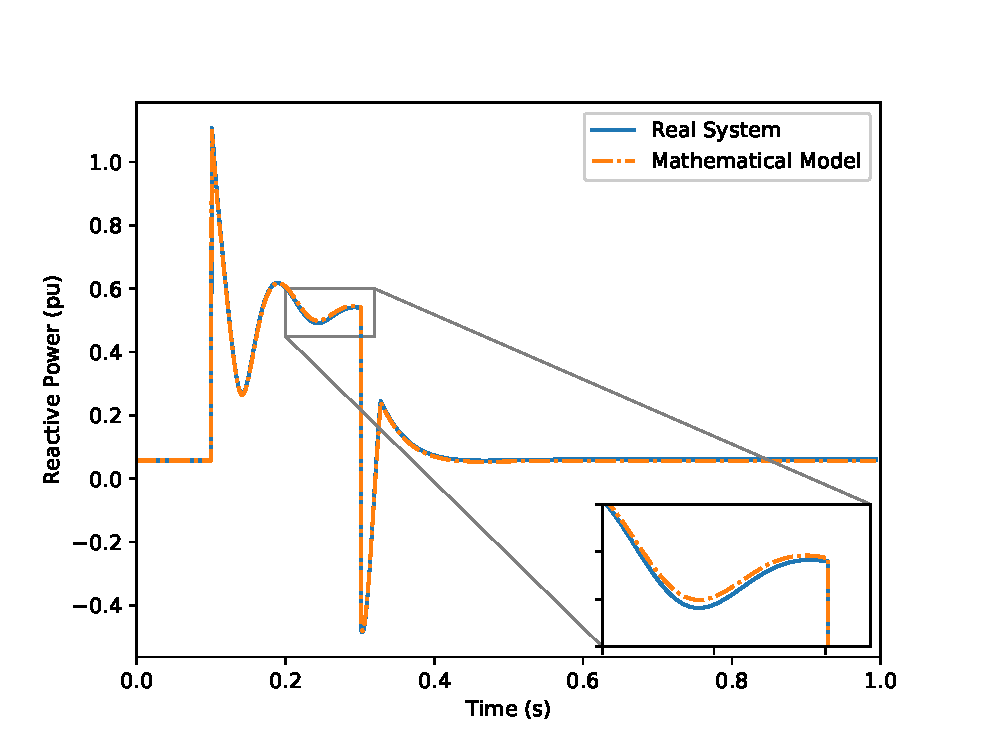
\includegraphics[scale=0.7]{Images/Q_compared.eps}
	\label{fig: output_Q}
\end{figure}

\subsection{Influence of MVMO Population Size}

In order to evaluate how the population size affects MVMO, a series of estimations using only this method were executed varying only the number of individuals. Five population sizes were chosen for this experiment (5, 10, 20, 50 and 100 individuals) and, for each one of them, 35 estimations were executed.

Apart from population size, all method configurations were fixed, so the results could be directly compared. The error tolerance was set at $tol_{1} = 0.5$ and the search region was the same as presented in Table \ref{tab: MVMO_boundaries}. The mean duration of estimation for each population size is shown below.

\begin{table}[h]
	\centering
	\caption{Influence of population size in MVMO}
	\begin{tabular}{c|c}
		\shortstack{\# of \\ individuals} & \shortstack{Mean \\ duration (s)} \\\hline
		5 & 15.62 \\
		10 & 11.08 \\
		20 & 13.02 \\
		50 & 17.84 \\
		100 & 29.00 
	\end{tabular}
	\label{tab: pop_size}
\end{table}

For considerably small populations (less than 5 individuals), the algorithm has to further explore the search region, due to reduced number of candidates. On the other extreme, large populations (more than 50 individuals) usually present good candidates in their initial population, only requiring a refinement of the solution. However, generating and evaluating all initial candidates has a huge cost, impacting on the estimation time. For these reasons, populations of 10 to 20 individuals present better convergence times than others, as depicted in Table \ref{tab: pop_size}.

\section{Simulation of Proposed Model}

Given the similarities between original and proposed models, the simulations of the latter were conducted using the same parameter values found for the former. It was observed that, in order to adjust the pre-fault behaviour of the proposed model, the upper limit of the delay blocks should be increased to at least $1.1$. With these changes made, the outputs of the proposed model were compared to the original WPP model, as displayed in Figures \ref{fig: proposed_P} and \ref{fig: proposed_Q}.

\begin{figure}[!h]
	\centering
	\caption{Active power from original and proposed models.}
	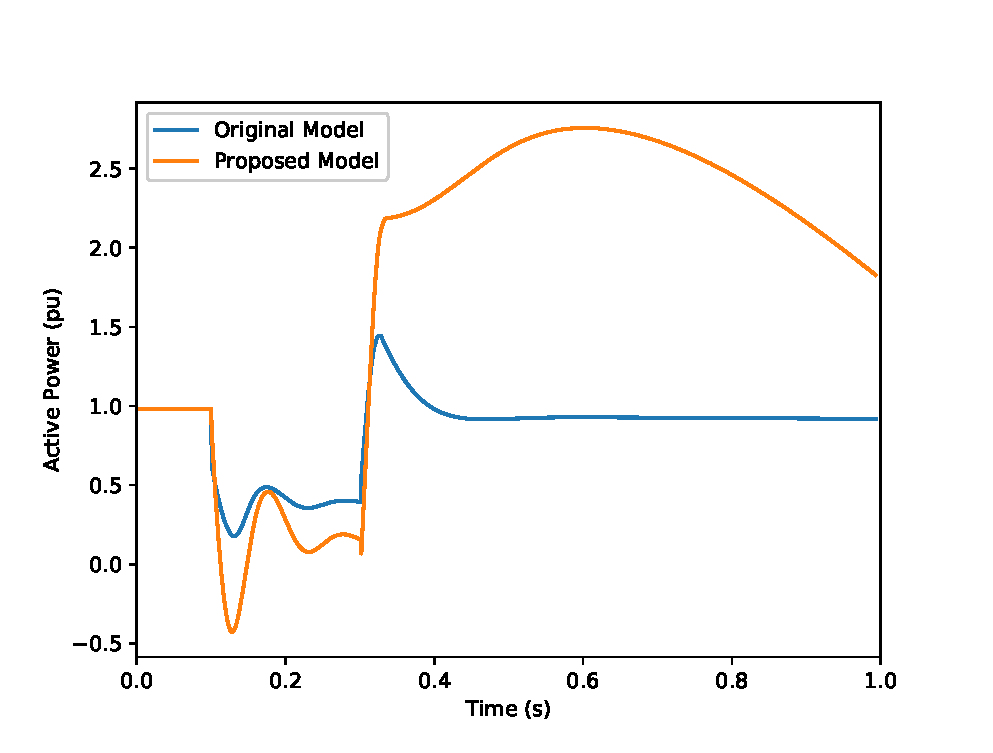
\includegraphics[scale=.7]{Images/P_proposed.eps}
	\label{fig: proposed_P}
\end{figure}

\begin{figure}[!h]
	\centering
	\caption{Reactive power from original and proposed models.}
	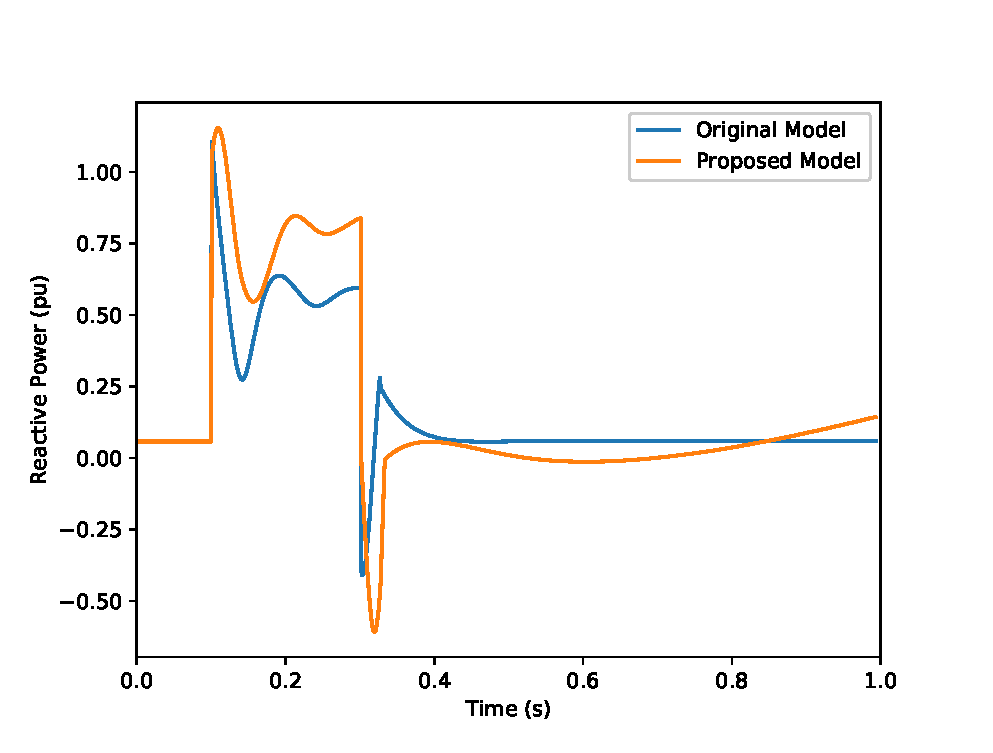
\includegraphics[scale=.7]{Images/Q_proposed.eps}
	\label{fig: proposed_Q}
\end{figure}

It can be noticed that reactive power calculated by the proposed model is not distant from the results obtained by the original WPP model. Active power, on the other hand, diverged from the expected, specially during post-fault. The parameter estimation for this model was conducted but could not find a solution, indicating that the proposed model is not entirely able to represent wind power plants yet, requiring further studies for improvement.
% ---
% Capítulo 6 - Conclusion
% ---
\chapter{Conclusion}
\label{ch: Conclusion}

In this work, a software for parameter estimation of mathematical models was developed and applied on a wind power plant model. The software created consists of framework and GUI, both developed in Python 3, where users can configure an estimation tool and select which models and methods it will be apply. For this application, two estimation methods were developed: MVMO, a population-based metaheuristic, and TSM, a non-linear method based on Newton-Raphson. However, new methods can be easily added to the framework as they are required.

Initial studies have shown that, by combining both MVMO and TSM, the estimation method obtained is able to perform better than both methods separately. This hybrid method initially applies MVMO in order to sweep the search region and provide a solution candidate close to the optimal values. The solution candidate provided by MVMO is then refined using TSM, which quickly reduces the error between model output and measurements. The combination of both approaches provides a robust and quick estimation method.

The software was then applied to estimate the parameters of a WPP model using the hybrid method mentioned above. For this application, the WPP model parameters can be estimated using measurement data of voltage angle and magnitude ($\phi_{v}$ and $v_{T}$) and active and reactive power ($P$ and $Q$) taken from the power plant terminal bus. Since measurements of voltage angle are needed by this model, the grid must contain special equipment, such as PMUs, installed on.

To avoid the requirement of voltage angle data and, thus, the installation of PMUs, a new model was proposed. This model, based on the one forementioned, would not need voltage angle measurements as input, allowing its application on a larger set of cases. However, initial tests on the proposed model were not successful and will be topic of ongoing research.

The software developed during the course of this work is available for download at \href{https://github.com/gnegrelli/identPy\_GUI}{https://github.com/gnegrelli/identPy\_GUI}.
% ---
% Capítulo 7 - Ongoing Research
% ---
\chapter{Ongoing Research}
\label{ch: Ongoing}

The estimation framework and GUI developed by the author and presented in this dissertation can be further improved in the future. New estimation methods, such as Kalman Filters, Monte Carlo, Particle Swarm Optimization and Differential Evolution, may be implemented to enlarge user options. Moreover, additional estimation steps, such as identifiability analysis, can be applied to validate and provide more information about the process. Further studies on the proposed WPP model are also needed in order to validate its application. Improvements on GUI may surface as other features are created and new users start applying the tool.
% ---
% Capítulo 8 - Publications
% ---
\chapter*{List of Publications}
\label{ch: Publications}

Below is presented a list of the publications generated during the course of this reasearch.

\begin{itemize}
	\item XXIII Congresso Brasileiro de Autom\'atica (2020) - "Parameter Estimation of Wind Power Plant Equivalent Model through a Hybrid Method"\footnote{To be published.}
	\item XIV Conferência Brasileira de Dinâmica, Controle e Aplicações (2019) - "Hybrid parameter estimation method for load model disturbed by OLTC"
	\item 2019 IEEE Canadian Conference of Electrical and Computer Engineering (2019) - "Load Model Identification Through a Hybrid Approach"
\end{itemize}
% ----------------------------------------------------------
% ELEMENTOS PÓS-TEXTUAIS
% ----------------------------------------------------------
\postextual
% ----------------------------------------------------------

% -----------------------------------------------------------
% Referências bibliográficas
% ----------------------------------------------------------
\bibliography{USPSC-modelo-references}

% ----------------------------------------------------------
% Glossário
% ----------------------------------------------------------
%
% Consulte o manual da classe abntex2 para orientações sobre o glossário.
%
%\glossary

% ----------------------------------------------------------
% Apêndices
% ----------------------------------------------------------
%% USPSC-Apendice.tex
% ---
% Inicia os apêndices
% ---

\begin{apendicesenv}
% Imprime uma página indicando o início dos apêndices
\partapendices

\chapter{Parameter Estimation of Spring-Mass Model}

The spring-mass system is a simple physical model often used as example of dynamic systems. It is composed of an object of mass $m$ connected to a fixed point in space by a spring of stiffness constant $k$. When disturbed by an external force $u$, the object oscillates and its movement is described by \eqref{eq: SpringMass}, $x$ is the position of the object while $x_{1}$ and $x_{2}$ correspond to its speed and acceleration, respectively. The system output, parameter vector, input and initial conditions are presented on \eqref{eq: SMoutput}, \eqref{eq: SMp}, \eqref{eq: SMinput} and \eqref{eq: SMinitcond}, respectively.

\begin{equation}
	\begin{bmatrix}
		\dot{x_{1}} \\
		\dot{x_{2}}
	\end{bmatrix} = 
	\begin{bmatrix}
		0 & 1 \\
		\frac{k}{m} & 0
	\end{bmatrix}\cdot
	\begin{bmatrix}
		x_{1} \\
		x_{2}
	\end{bmatrix} -
	\begin{bmatrix}
		0 \\
		\frac{1}{m}
	\end{bmatrix}
	\cdot
	u
	\label{eq: SpringMass}
\end{equation}

\begin{equation}
	y = \begin{bmatrix}
		x_{1}, x_{2}
	\end{bmatrix}^ {T}
	\label{eq: SMoutput}
\end{equation}

\begin{equation}
	p = \begin{bmatrix}
		m, k
	\end{bmatrix}^ {T}
	\label{eq: SMp}
\end{equation}

\begin{equation}
	u(t = 0) = 1
	\label{eq: SMinput}
\end{equation}

\begin{equation}
	\begin{cases}
		x_{1}(0) = 0 \\
		x_{2}(0) = 0
	\end{cases}
	\label{eq: SMinitcond}
\end{equation}

The behaviour of the real system was obtained by means of simulation with parameters set at $m = 3\ kg$ and $k = 6\ N/m$. Three different estimation process were executed: TSM, MVMO and the hybrid approach of MVMO and TSM combined. The tolerance for all three estimations was set at $tol = 0.1$.

\section{Trajectory Sensitivity Results}

It took only 7 iterations (7 seconds on a PC) for Trajectory Sensitivity Method to estimate the parameters when the initial values were $m_{0} = 7\ kg$ and $k_{0} = 7\ N/m$. This shows how fast this method is, as long as the initial values are in the neighbourhood of the real parameters. Figure \ref{fig: TS_conv} shows the error evolution during estimation suing TSM.

\begin{figure}[h]
	\caption{Error evolution of TSM with $m_{0} = 7\ kg$ and $k_{0} = 7\ N/m$}
	\begin{center}
		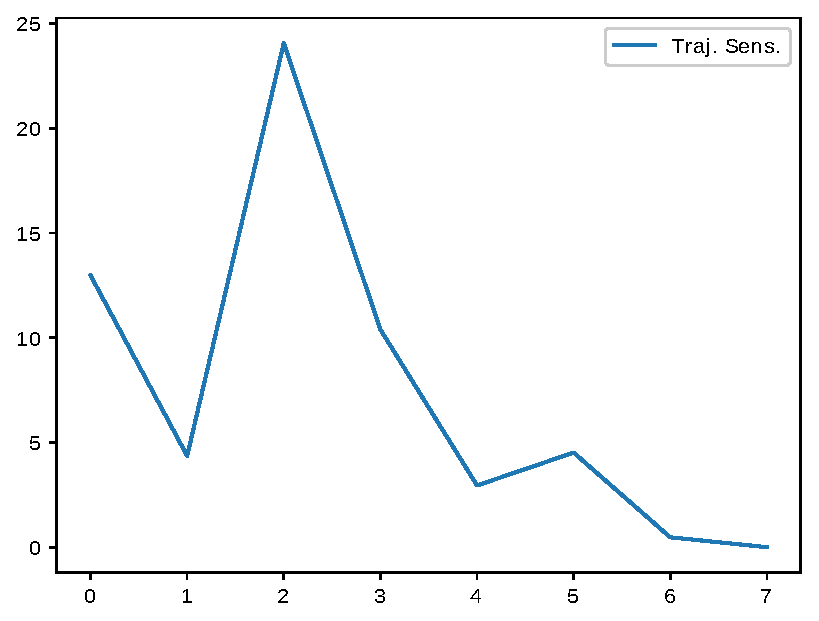
\includegraphics[scale=0.7]{Images/TS_conv.eps}
	\end{center}
	\label{fig: TS_conv}
\end{figure}

However, the convergence region \footnote{Convergence region is a region in parameter space where, if the initial guess for parameter values is inside it, the convergence to true values is guaranteed.} of TSM is extremely limited, diverging for initial points far enough from the real values. The convergence region for the real values was obtained in \cite{Ecyo} and is shown in Figure \ref{fig: conv_reg}. For comparison, the MVMO and the hybrid approach converge for the entire search region displayed on the graph.

\begin{figure}[h]
	\caption{Convergence region of Trajectory Sensitivity Method}
	\begin{center}
		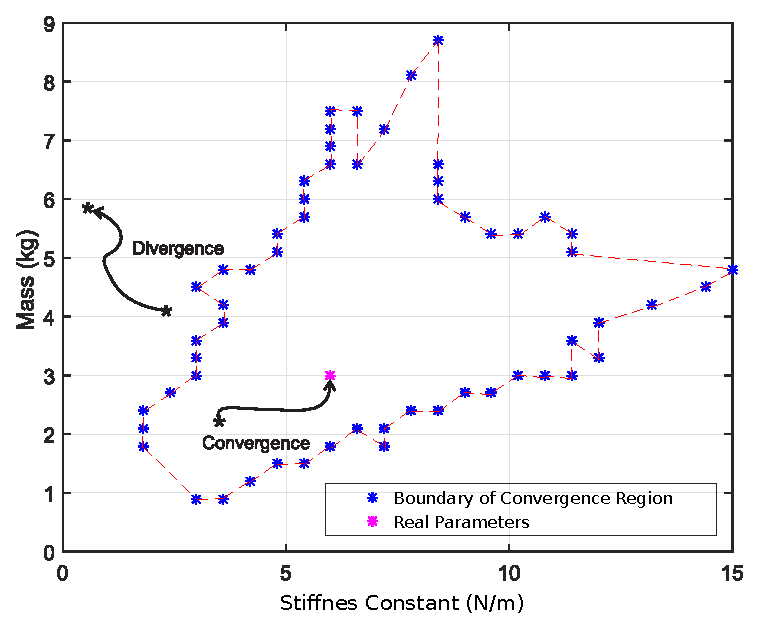
\includegraphics[scale=0.7]{Images/Conv_reg.eps}
	\end{center}
	\label{fig: conv_reg}
	\legend{Source: Adapted from \cite{Ecyo}}
\end{figure}

To illustrate the importance of good initial values, the parameters were reestimated using TSM, but now the initial values were set to be $m_{0} = 8\ kg$ and $k_{0} = 10\ N/m$. Notice that these values are not too far from the ones used in the previous estimation. The results, on the other hand, were extremely different. The method was not able to lower the error below $16.4$ and the parameters found were $m_{f} = 2.7\ kg$ and $k_{f} = 118.6\ N/m$. The error evolution for this estimation is depict in Figure \ref{fig: TS_nconv}.

\begin{figure}[h]
	\caption{Error evolution of TSM with $m_{0} = 8\ kg$ and $k_{0} = 10\ N/m$}
	\begin{center}
		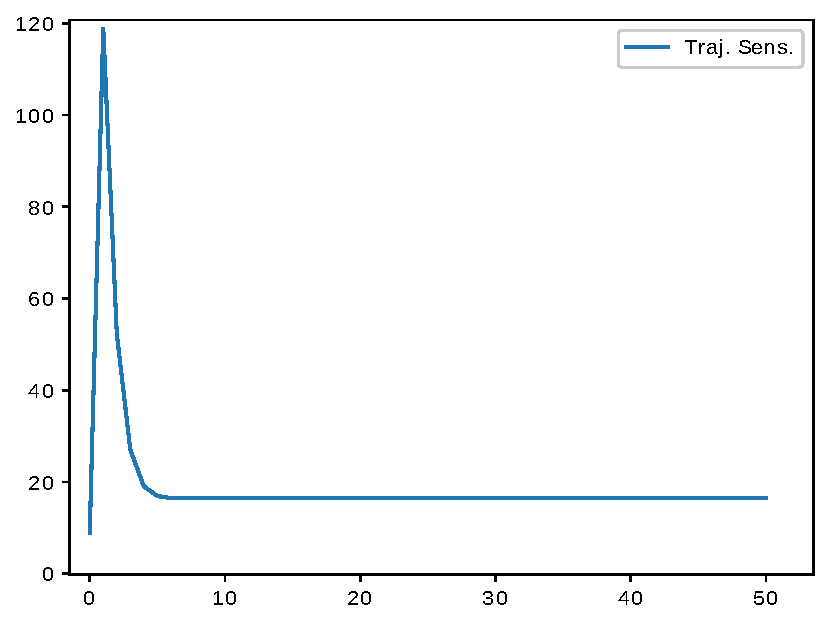
\includegraphics[scale=0.7]{Images/TS_nconv.eps}
	\end{center}
	\label{fig: TS_nconv}
\end{figure}

\section{MVMO Results}

To use MVMO, a search region in parameter space must be defined. Therefore, the parameters boundaries was defined as $0 \leq m \leq 9$ and $0 \leq k \leq 15$. The population size was set at 5 individuals and after every generation 1 new individual was created. The heuristic method converged after almost 10000 generations, as depicted in Figure \ref{fig: MVMO_conv}. This figure also shows how MVMO rapidly reduces error of estimation, but as the values approach the neighbourhood of the real values, it slows down.

\begin{figure}[h]
	\caption{Error evolution of MVMO}
	\begin{center}
		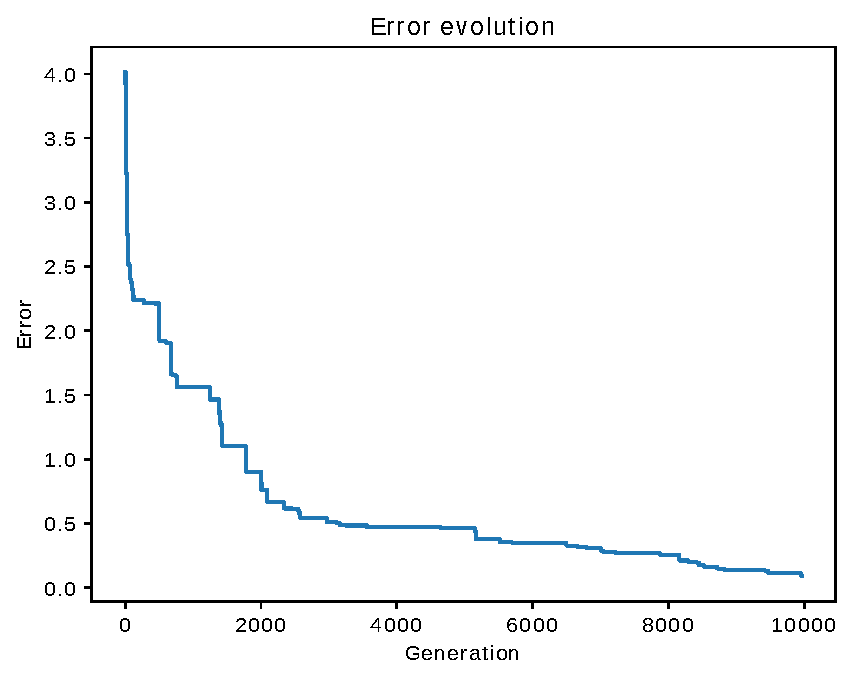
\includegraphics[scale=0.7]{Images/MVMO_conv.eps}
	\end{center}
	\label{fig: MVMO_conv}
\end{figure}

\section{Hybrid Approach Results}

By combining both methods, the hybrid approach benefits from the quick error reduction provided by MVMO and the fast convergence from TSM when inside convergence region. The error evolution obtained from this approach is depicted in Figure \ref{fig: Hybrid_conv}. The tolerance for this approach were set at $tol_{1} = 1.5$ and $tol_{2} = 0.1$.

\begin{figure}[h]
	\caption{Results of hybrid approach for spring-mass system}
	\begin{center}
		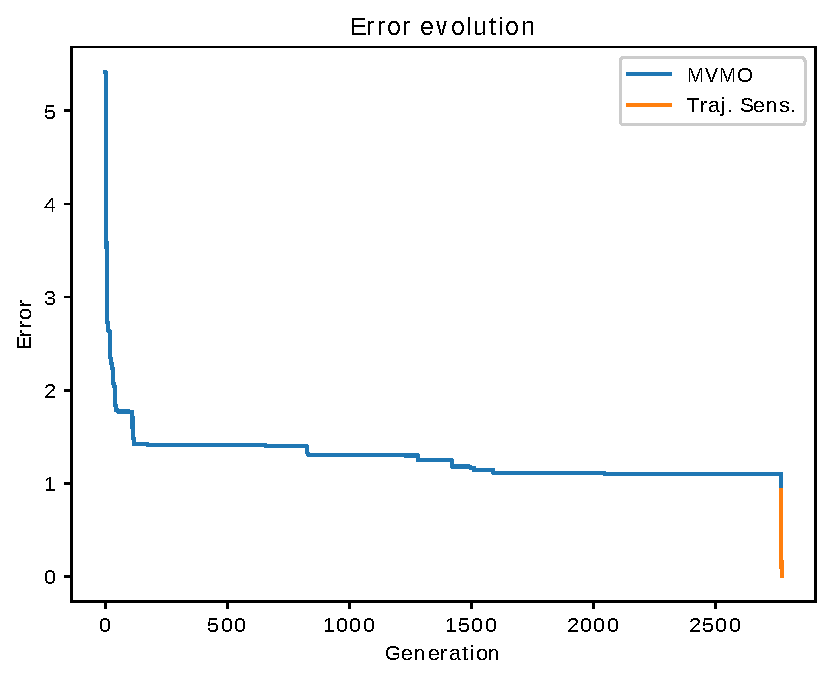
\includegraphics[scale=0.7]{Images/Hybrid_conv.eps}
	\end{center}
	\label{fig: Hybrid_conv}
\end{figure}

When compared to each method, the hybrid approach converges faster than MVMO but slower than TSM, as shown in Table \ref{tab: SM}. Although all methods converged to parameter values that resulted in an error level below the tolerance, TSM and the Hybrid approach provided final results with error level below the values obtained by MVMO.

\begin{table}[h]
	\caption{Comparison of approaches}
	\begin{center}
	\begin{tabular}{c|c|c}
		Approach & Time & Final Error \\
		\hline
		TSM  & $7 \ s$  & $2.76\times 10^{-3}$ \\
		MVMO  & $24 \ min$  & $89.33\times 10^{-3}$\\
		Hybrid  & $10 \ min$  & $1.54\times 10^{-3}$
	\end{tabular}
	\end{center}
	\label{tab: SM}
\end{table}

%------------------------------------------------------------
\chapter{Parameter Estimation of Linearized Z-IM Load Model}

The hybrid approach was also employed on parameter estimation of Z-IM Load Model. This model is able to predict the behaviour of electrical loads during faults in the grid. The Z-IM Load Model is composed of an impedance in parallel with a third-order induction motor (IM), as shown in Figure \ref{img: Z-IM}. According to \cite{Choi}, this model results in low error levels for both active and reactive power, alongside having a smaller parameter vector when compared with other models. It is described by the following equations:

\begin{figure}[h]
    \caption{Schematic of Z-IM Load Model.}
    \begin{center}
    	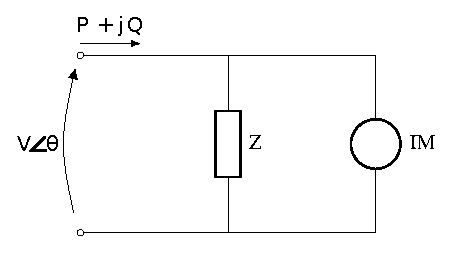
\includegraphics[scale=1]{Images/drawZIM.eps}
    \end{center}
    \label{img: Z-IM}
\end{figure}

\begin{equation}
    \begin{cases}
        \dot{\Delta E'} = \frac{-1}{T_{o}X'}[X\Delta E' + (X - X')V_{0}\sin\delta_{0}\Delta \delta] + \frac{(X - X')\cos\delta_{0}}{T_{0}X'}\Delta V \\
        \\
        \dot{\Delta \delta} = \frac{(X-X')V_{0}}{T_{0}X'E'_{0}}\cdot\left(\frac{\sin\delta_{0}\Delta E'}{E'_0} - \cos\delta_{0}\Delta\delta\right) + \Delta\omega - \frac{(X - X')\sin\delta_0}{T_o X'E'_0}\Delta V \\
        \\
        \dot{\Delta \omega} = \frac{-V_{0}}{MX'}(\sin\delta_{0}\Delta E' + E'_{0}\cos\delta_{0}\Delta\delta) - \frac{E'_0\sin\delta_0}{MX'}\Delta V
    \end{cases}
    \label{eq: xZIM}
\end{equation}

\begin{equation}
    \begin{cases}
        \Delta P = \frac{-V_{0}}{X'}(\sin{\delta_{0}}\Delta E' + E'_{0}\cos{\delta_{0}}\Delta \delta) + \left(2G_{s} V_{0} - \frac{E'_{0} \sin{\delta_{0}}}{X'}\right)\Delta V \\
        \\
        \Delta Q = \frac{-V_{0}}{X'}(\cos{\delta_{0}}\Delta E' + E'_{0}\sin{\delta_{0}}\Delta\delta) + \left(2B_{s} V_{0} + \frac{2V_{0} - E'_{0} \cos{\delta_{0}}}{X'}\right)\Delta V
    \end{cases}
    \label{eq: yZIM}
\end{equation}

\begin{equation}
    \begin{cases}
    X = X_{s} + X_{m} \\
    X' = X_{s} + \frac{X_{m} X_{r}}{X_{m} + X_{s}} \\
    T_{o} = \frac{X_{r} + X_{m}}{\omega_{s} R_{r}}
    \end{cases}
    \label{eq: terms}
\end{equation}

\noindent where the terms $\Delta E'$ and $\Delta \delta$ represent the variation on voltage magnitude and angle at the motor terminals, $\Delta \omega$ is the variation on stator speed, in rad/s. $X_m$, $X_s$ and $X_r$ are the magnetizing, stator and rotor reactances, respectively, $R_r$ stands for the rotor resistance, $\omega_{s}$ is the synchronous speed, $T_o$ represents the open-circuit transient time constant, $M$ is the motor inertia and $V_{0}$ is the voltage on the load terminals before the disturbance. The state, output, input and parameter vectors are presented in \eqref{eq: ZIMstate}, \eqref{eq: ZIMoutput}, \eqref{eq: ZIMinput} and \eqref{eq: ZIMparam}, respectively.

\begin{equation}
	x = [\Delta E', \Delta \delta, \Delta \omega]^{T}
	\label{eq: ZIMstate}
\end{equation}

\begin{equation}
	y = [\Delta P, \Delta Q]^{T}
	\label{eq: ZIMoutput}
\end{equation}

\begin{equation}
	u = [\Delta V]
	\label{eq: ZIMinput}
\end{equation}

\begin{equation}
	p = [X, X', T_{0}, M, G_{s}, B_{s}, E'_{0}, \delta_{0}]^{T}
	\label{eq: ZIMparam}
\end{equation}

The Z-IM load model is much more complex than the spring-mass system, with 9 parameters to be estimated. The hybrid approach proposed was able to estimate the parameters of this system and the comparison between real and modeled behaviour with the parameters obtained can be seen in the Figure \ref{fig: ZIM}.

\begin{figure}[h]
	\caption{Result of parameter estimation for Z-IM Load Model}
	\begin{center}
		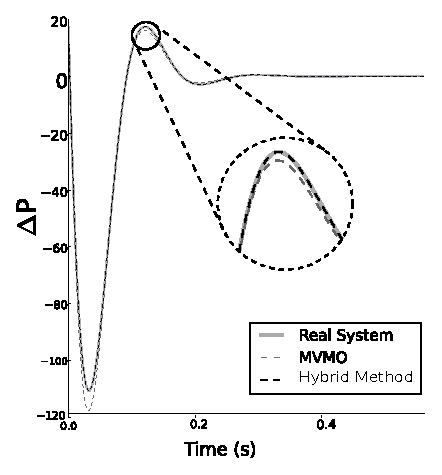
\includegraphics[scale=1]{Images/ZIM.eps}
	\end{center}
	\label{fig: ZIM}
	\legend{Source: \cite{Gomes2019}}
\end{figure}

The application of the hybrid approach on Linearized Z-IM Load Model is subject of a paper presented by the author on the 2019 IEEE Canadian Conference on Electrical and Computer Engineering entitled ``\textit{Load Model Identification Through a Hybrid Approach}".
% ---
\end{apendicesenv}

% ----------------------------------------------------------
% Anexos
% ----------------------------------------------------------
%%% USPSC-Anexos.tex
% ---
% Inicia os anexos
% ---
\begin{anexosenv}

% Imprime uma página indicando o início dos anexos
\partanexos

% ---
\chapter{Exemplo de anexo}
% ---
Elemento opcional, que consiste em um texto ou documento não elaborado pelo autor, que serve de fundamentação, comprovação e ilustração, conforme a ABNT NBR 14724. \cite{nbr14724}.

O \textbf{ANEXO B} exemplifica como incluir um anexo em pdf.

\chapter{Acentuação (modo texto - \LaTeX)}
\begin{figure}[H]
	\begin{center}
	\caption{\label{fig_anexob}Acentuação (modo texto - \LaTeX)}
	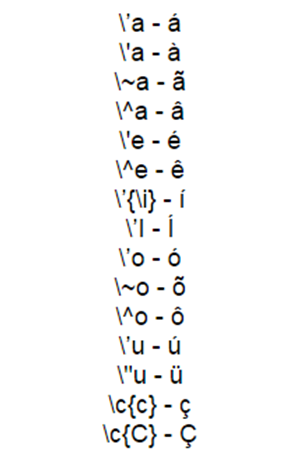
\includegraphics[scale=1.0]{USPSC-AcentuacaoLaTeX.png} \\
	Fonte: \citeonline{comandos}
	\end{center}	
\end{figure}

\chapter{Símbolos úteis em \LaTeX}
\begin{figure}[H]
	\begin{center}
		\caption{\label{fig_anexoc}Símbolos úteis em \LaTeX}
		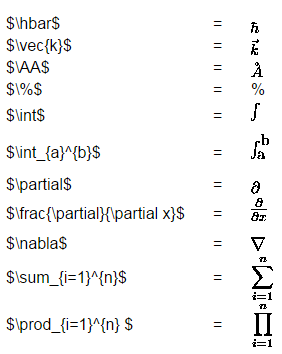
\includegraphics[scale=1.0]{USPSC-SimbolosUteis.png} \\
		Fonte: \citeonline{comandos}
	\end{center}	
\end{figure}


\chapter{Letras gregas em \LaTeX}
\begin{figure}[H]
	\begin{center}
		\caption{\label{fig_anexod}Letras gregas em \LaTeX}
		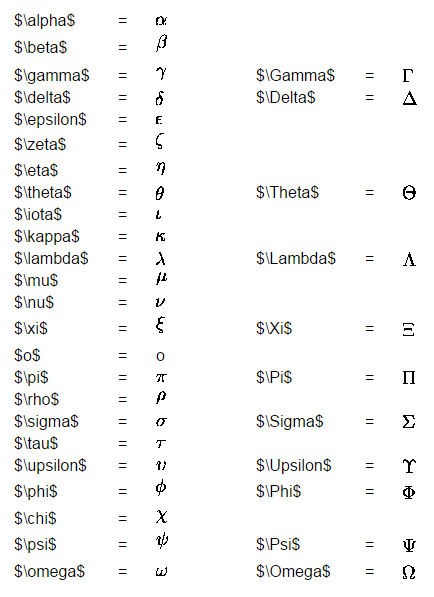
\includegraphics[scale=1.0]{USPSC-LetrasGregas.png} \\
		Fonte: \citeonline{comandos}
	\end{center}	
\end{figure}

\end{anexosenv}


%---------------------------------------------------------------------
% INDICE REMISSIVO
%--------------------------------------------------------------------
\phantompart
\printindex

%---------------------------------------------------------------------

\end{document}
